\documentclass[a4paper,12pt, openright]{report}
\usepackage[utf8]{inputenc}
\usepackage{hyperref}
\usepackage{url}
\usepackage{natbib}
\usepackage{graphicx}
\usepackage{enumitem}
\usepackage{cleveref}
\usepackage{tabularx}
\usepackage{enumitem}
\setenumerate{label*=\arabic*.}

\usepackage{mytodonotes}

\newcommand{\emailaddr}[1]{\href{mailto:#1}{\texttt{#1}}}


\title{Project Management Report}
\author{
    Mattia Matteini \\ \emailaddr{mattia.matteini@studio.unibo.it}
    \and
    Alberto Paganelli \\ \emailaddr{alberto.paganelli3@studio.unibo.it}
    \and
    Giacomo Totaro \\ \emailaddr{giacomo.totaro2@studio.unibo.it}
}

\date{July 2024}

\begin{document}

\maketitle

\tableofcontents

\clearpage

%\setcounter{chapter}{1}

\chapter{Introduzione}
In questo documento, viene presentato l'approccio intrapreso per la simulazione di gestione di un progetto. Esso sarà basato sulle best-practice viste durante il corso di Project Management.
I capitoli successivi seguono il tipico ordine dei gruppi di processo: si inizia con una fase di scoping e si termina con la chiusura del progetto.
Le seguenti sezioni di questo capitolo forniscono informazioni generali relative all’azienda esecutrice e a quella committente.

\section{Analisi del dominio}

Il campo delle perizie è da sempre un settore molto competitivo, dove se non rimani al passo attraverso digitalizzazione o riallineamento con i vari competitor potrebbe scaturire qualche rischio, proprio come in questo caso. I principali soggetti coinvolti sono le compagnie di assicurazione, periti e clienti.
Ogni studio peritale autonomo si interpone tra il cliente e la compagnia di assicurazione, fornendo valutazioni dei danni e stima dei costi.
Le compagnie, basandosi su efficienza e accuratezza delle perizie, scelgono gli studi con cui collaborare. 
L'efficienza è un fattore chiave per la scelta di uno studio peritale, in quanto una perizia rapida e accurata permette alla compagnia di assicurazione di risparmiare tempo, denaro ed ottenere guadagni anche in termini di immagine. Non sempre però ciò accade anche per gli studi peritali, che per accaparrarsi una buona posizione nel mercato delle perizie, offrono servizi a prezzi molto competitivi, riducendo i margini di profitto.
La problematica che ha richiesto l'intervento di un team di consulenti è legata alla mancanza di efficienza dei processi interni dello studio peritale X. In particolare, si è riscontrato che i processi di perizie relative a sinistri minori sono inefficienti e non rispettano i tempi di consegna previsti. Questo ha portato ad un calo significativo del margine di profitto dello studio peritale (35\%) che se non riesce a risolvere il problema rischia di perdere la collaborazione con alcune maggiori compagnie assicurative e quindi di dover ridurre drasticamente il proprio personale.

\chapter{Scoping}
In questa sezione si riportano le scelte intraprese durante lo scoping, iniziando con una breve descrizione sul come sia avvenuto il primo contatto tra le due aziende. Per maggior chiarezza, vengono elencati i principali \textit{deliverables} che tale fase deve produrre:
\begin{itemize}
    \item Resource Breakdown Structure (RBS)
    \item Project Overview Statement (POS)
\end{itemize}

\section{Primo contatto}
Il primo contatto è avvenuto in modo informale, con la richiesta di un possibile progetto comunicata a un membro del team. In seguito, questa comunicazione informale è stata approfondita attraverso una serie di email e telefonate, che hanno consentito di chiarire gli obiettivi iniziali e le aspettative di entrambe le parti. Mostrando interesse per la proposta, il team ha quindi deciso di organizzare un Process Scoping Meeting. Questo incontro è stato pianificato per delineare lo scope del progetto, eliminare eventuali ambiguità e, soprattutto, valutare attentamente la fattibilità della proposta.

\subsection{Ubiquitous Language}
Vedi tabella \ref{tab:ubiquitous-language}
\begin{table}
        \centering
        \begin{tabularx}{1\textwidth}{ | c | >{\centering\arraybackslash}X | }
            \hline
            \textbf{Termine} & \textbf{Significato} \\
            \hline
            Cliente & Studio peritale X che ha richiesto l'intervento di un team di consulenti per risolvere la problematica legata alla mancanza di efficienza dei processi interni. \\
            \hline
            Studio peritale & Studio specializzato nella valutazione dei danni e nella stima del danno. Dispone di un'equipe di periti che si muovono nella zona coperta dallo studio, ognuno con determinate specializzazioni. \\
            \hline
            Assicurato & Persona fisica o giuridica che ha stipulato una polizza assicurativa e che, nel caso di sinistro, ha diritto ad una perizia per la valutazione del danno e del conseguente risarcimento. \\
            \hline
            Polizza & Contratto di assicurazione stipulato tra l'assicurato e la compagnia assicurativa che garantisce la copertura dei danni in caso di sinistro. \\
            \hline
            Compagnia & Compagnia assicurativa che ha stipulato la polizza con il cliente. Essa delega agli studi peritali lo svolgimento delle perizie.
            \\
            \hline
            Incarico & Insieme di attività che vengono svolte dallo studio peritale per conto della compagnia assicurativa. L'incarico solitamente è relativo ad un singolo sinistro e, tra le altre cose, prevede la valutazione del danno e la stima del risarcimento. \\
            \hline
            Sinistro & Evento che causa un danno all'assicurato e che richiede l'intervento della compagnia assicurativa per la valutazione del danno e la stima del risarcimento. Corrisponde poi ad un incarico per lo studio peritale \\
            \hline
            Perito & Persona incaricata dallo studio peritale per effettuare le perizie. \\
            \hline
            Georeferenziare & Processo di associazione di informazioni geografiche a un oggetto, in questo caso ad un'immagine. Queste informazioni sono contenute nei metadati dell'immagine e permettono di localizzare il luogo in cui è stata scattata l'immagine onde evitare errori di valutazione del danno o truffe da parte dell'assicurato \\
            \hline
        \end{tabularx}
        \caption{Ubiquitous Language}
        \label{tab:ubiquitous-language}
    \end{table}


\subsection{Conditions of Satisfation (CoS)}
Dalle richieste del committente, emerse durante la prima ``chiacchierata'', il team ha individuato le seguenti \textbf{Condition of Satisfaction}, che rappresentano le aspettative chiave del cliente e del progetto:
\begin{itemize}
    \item \textbf{Tempo di completamento degli incarichi}: Entro un anno dall'implementazione, ottimizzando i processi interni dello studio peritale e aumentando l’efficienza delle perizie relative a sinistri minori, il sistema deve abbattere le problematiche relative ai sinistri minori salvo eccezione di casi particolari;
    \item \textbf{Aumento di sinistri presi in carico}: Si prevede, come conseguenza del punto precedente, un aumento del 15\% della gestione di nuovi incarichi;
    \item \textbf{Vincoli di budget}: Il progetto deve essere portato a termine rientrando nel budget previsto per la sua esecuzione, che ammonta a 50.000€, considerando nel caso peggiore, una tolleranza pari al ``sesto quinto'';
    \item \textbf{Vincoli di tempo}: Portare a termine il progetto rientrando nelle tempistiche previste, in particolare, a causa della digitalizzazione del mercato (e della concorrenza), si vuole avere una soluzione funzionante entro Ottobre dell'anno corrente;
    \item \textbf{Soddisfazione dei periti nell'utilizzo del sistema}: Il prodotto software deve fornire un'interfaccia utente intuitiva garantendo un'ottima esperienza utente;
    \item \textbf{Conformità normativa}: Assicurare che il sistema sia conforme alle normative vigenti sulla privacy e sicurezza dei dati, garantendo la protezione dei dati personali dei clienti e delle compagnie assicurative;
    \item \textbf{Documentazione completa del software}: La documentazione deve essere chiara e consultabile nel caso in cui siano necessari chiarimenti;
    \item \textbf{Integrazione}: Garantire che il nuovo sistema sia completamente integrato con i sistemi informatici degli studi peritali, consentendo il trasferimento automatizzato di dati;
    \item \textbf{Formazione del personale}: Formare il 100\% del personale dello studio peritale sull'utilizzo del nuovo sistema entro tre mesi dall'implementazione, al fine di massimizzare l'adozione e l'efficacia del sistema.
\end{itemize}


\section{Primo project scoping meeting}
Nel primo incontro di project scoping hanno partecipato l'intero team esecutivo, un Project Manager e un esperto del dominio dell'azienda committente. Data l'importanza e la complessità dei concetti sottostanti su cui si basa questo progetto, è stato essenziale acquisire una comprensione approfondita del dominio. Inizialmente, non è stata stabilita un'agenda rigida, ma è stato richiesto di fornire documentazione che il team avrebbe dovuto esaminare prima del prossimo incontro, permettendo così domande più mirate nelle fasi successive. Durante questa riunione, il team ha presentato alcune possibili soluzioni al problema e alla fine sono state discusse ed aggiornare le ``Conditions of Satisfaction (CoS)'' in base alle nuove informazioni.

\subsection{Project Overview Statement}
Successivamente al primo meeting, è stato redatto il documento ``Project Overview Statement'' seguito da un'analisi dei rischi per comprendere meglio le possibili criticità del progetto.

\subsubsection{Problem/Opportunity}
Lo studio peritale X ha subito un calo del margine di profitto del 35\% a causa di una mancanza di efficienza nei processi interni, in particolare per le perizie relative a sinistri minori. Questi sinistri rappresentano una significativa quota di mercato con margini di guadagno relativamente bassi per lo studio, ma sono fondamentali per garantire buone performance alle compagnie assicurative e ottenere lavori più remunerativi.

\subsubsection{Project Goal}
Implementare un sistema innovativo per la gestione delle perizie di sinistri minori presso lo studio peritale X, ottimizzando i processi interni per garantire efficienza, rapidità e qualità nel servizio offerto alle compagnie assicurative. L'obiettivo è aumentare i margini di profitto, consentendo ai periti di gestire un volume maggiore di perizie minori in meno tempo, al fine di consolidare la fiducia delle compagnie assicurative.

\subsubsection{Project Objectives}
Gli obiettivi sono:
\begin{enumerate}
    \item Creare un processo semplificato per la gestione delle perizie di sinistri minori;
    \item Implementare un sistema di gestione delle perizie che permetta di effettuare perizie da remoto;
    \item Implementare un sistema di gestione incarichi per i periti;
    \item Aumentare la qualità del servizio offerto alle compagnie assicurative e ai clienti misurando la soddisfazione tramite questionari di valutazione;
    \item Fornire alle compagnie assicurative un sistema di monitoraggio delle perizie in tempo reale attraverso un'interfaccia del sistema.
\end{enumerate}

\subsubsection{Success Criteria}
\begin{itemize}
    \item Recupero del 35\% di perdite entro un anno;
    \item Aumento del margine di profitto del 10\% entro due anni;
    \item Aumento della qualità del servizio offerto alle compagnie assicurative e ai clienti;
    \item Aumento di sinistri minori gestiti del 50\% entro un anno;
    \item Ritorno alla competitività del mercato entro un anno.
\end{itemize}


\subsubsection{Assunzioni}
\begin{itemize}
    \item Sono disponibili le infrastrutture necessarie come postazioni desktop complete di cuffie, microfoni, webcam e una buona connessione internet;
    \item L'assicurato dispone di una connessione internet sufficientemente veloce;
    \item Il sistema rispetterà vincoli tecnologici e di sicurezza imposti dalle compagnie assicurative;
    \item Il personale dello studio peritale X sarà formato all'utilizzo del nuovo sistema.
\end{itemize} 
\subsubsection{Rischi}
\begin{itemize}
    \item Il personale potrebbe non essere in grado di utilizzare il nuovo sistema anche a seguito di formazione;
    \item Lo studio peritale potrebbe non essere in grado di gestire il nuovo carico di lavoro, richiedendo l'assunzione di nuovo personale o il cambio di organizzazione interna generando costi aggiuntivi;
    \item Il sistema per poter essere utilizzato dovrà rispettare i vincoli di data privacy e sicurezza dei dati personali imposti dalle normative vigenti e dalle compagnie assicurative;
    \item Il sistema potrebbe non essere compatibile con i sistemi informatici delle compagnie assicurative;
    \item Tenere in considerazione il fatto che la perizia non si svolge in presenza e di conseguenza l'accuratezza potrebbe non risultare ottimale.
\end{itemize}
\subsubsection{Ostacoli}
\begin{itemize}
    \item La creazione di un sistema in grado di svolgere video-perizie richiede la gestione di complessità tecnica significativa che dovrà essere totalmente gestita dal team e risultare trasparente al cliente;
    \item Agli utenti finali del sistema, da ambo le parti, dovrà poter essere garantita una user experience ottimale prediligendo la facilità d'uso, dettaglio non sempre facilmente ottenibile visto le numerose funzionalità che dovranno essere presenti. 
\end{itemize}

\subsection{Analisi dei Rischi}

Successivamente vengono analizzati più nel dettagli i rischi brevemente elencati nel POS. Tali rischi sono classificati usando una matrice di rischio (\cref{fig:risk}), e viene proposta una possibile mitigazione per ognuno di essi.

\begin{figure}[ht]
    \centering
    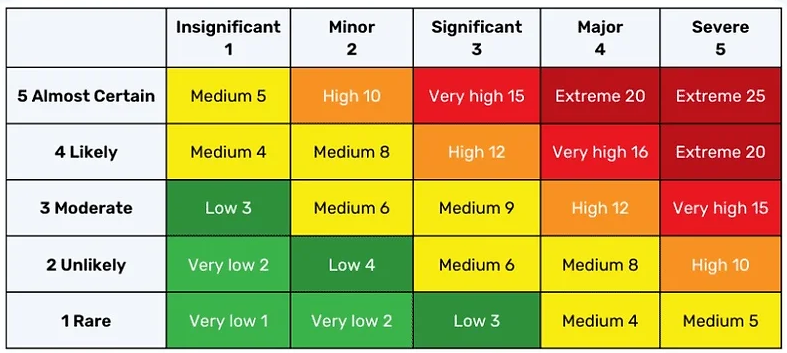
\includegraphics[width=14cm]{img/Tab_rischi.jpg}
    \caption{Matrice di rischio}
    \label{fig:risk}
\end{figure}

\begin{enumerate}
    \item \textbf{Difficoltà di utilizzo del sistema}: Il personale potrebbe non essere in grado di utilizzare il nuovo sistema anche a seguito di formazione.
    \\
    \textbf{Stima}: Medio (9)
    \\
    \textbf{Possibile mitigazione}: Implementare un programma di formazione continua, offrire supporto tecnico dedicato e video tutorial.

    \item \textbf{Gestione del carico di lavoro}: Lo studio peritale potrebbe non essere in grado di gestire il nuovo carico di lavoro, richiedendo l'assunzione di nuovo personale o il cambio di organizzazione interna generando costi aggiuntivi.
    \\
    \textbf{Stima}: Alto (12)
    \\
    \textbf{Possibile mitigazione}: Pianificare una fase di assunzione e formazione graduale del nuovo personale e ottimizzare il sistema di gestione del carico di lavoro per distribuire equamente le attività tra i periti.

    \item \textbf{Conformità privacy e sicurezza}: Il sistema per poter essere utilizzato dovrà rispettare i vincoli di data privacy e sicurezza dei dati personali imposti dalle normative vigenti e dalle compagnie assicurative.
    \\
    \textbf{Stima}: Molto alto (15)
    \\
    \textbf{Possibile mitigazione}: Collaborare con esperti di sicurezza informatica e consulenti legali per garantire la conformità alle normative e implementare misure di sicurezza avanzate.

    \item \textbf{Compatibilità}: Il sistema potrebbe non essere compatibile con i sistemi informatici delle compagnie assicurative.
    \\
    \textbf{Stima}: Medio (8)
    \\
    \textbf{Possibile mitigazione}: Mantenere una comunicazione costante con le compagnie assicurative per risolvere eventuali problemi di compatibilità e sviluppare API per garantire l'integrazione senza problemi. 

    \item \textbf{Accuratezza delle perizie remote}: Tenere in considerazione il fatto che la perizia non si svolge in presenza e di conseguenza l'accuratezza potrebbe non risultare ottimale.
    \\
    \textbf{Stima}: Basso (4)
    \\
    \textbf{Possibile mitigazione}: Utilizzare strumenti tecnologici avanzati, come immagini ad alta risoluzione e video in tempo reale, per migliorare l'accuratezza delle perizie remote e introdurre controlli di qualità aggiuntivi per verificare la precisione delle perizie remote.
\end{enumerate}

\section{Secondo project scoping meeting}
Nel secondo incontro di project scoping, è stato coinvolto nuovamente il project manager insieme a un esperto del dominio dell'azienda committente, oltre all'intero team esecutivo. L'obiettivo principale era quello di perfezionare ulteriormente i requisiti del progetto. Inizialmente, è stato richiesto agli esperti del dominio di esaminare attentamente i documenti esistenti per verificare la correttezza delle definizioni e dei concetti. Successivamente, sono state formulate ulteriori domande per chiarire gli aspetti critici delle funzionalità che il nuovo sistema dovrà incorporare. Durante questo incontro, è stato avviato lo sviluppo di una bozza della ``Requirement Breakdown Structure'' (RBS), che costituirà una mappa dettagliata dei requisiti del progetto.

\subsection{Requirement Breakdown Structure}
Le metodologie seguite per la defizione dei requisiti sono state le interviste e osservazioni sul campo. In un dominio nel quale nessuno di noi aveva esperienza, abbiamo ritenuto che la raccolta dei requisiti tramite queste due metodologie fosse il metodo più efficace e veloce per comprendere a fondo il dominio, problema e le particolari esigenze del cliente. Avendo la possibilità di fare domande si è cercato di capire, molto indicativamente, anche il carico di lavoro che dovremmo supportare. 
Un aspetto positivo di questo approccio è che ci ha consentito di capire quali fossero, oltre ai principali problemi, i desiderata del cliente potendo puntare a una situazione di early win. 

\subsubsection{Esempio intervista}
Di seguito un esempio di intervista effettuata al personale dello studio peritale, partendo dagli amministratori fino agli end-user.

\begin{enumerate}
    \item Quali sono le principali sfide che il vostro team affronta durante la gestione delle perizie di sinistri minori?
    \item Quali competenze specifiche sono richieste al personale per svolgere perizie accurate ed efficienti? Queste ultime, cambiano sulla base della tipologia di sinistro?
    \item In base a che cosa attribuite un incarico ad uno specifico perito? 
    \item Quanto tempo dedicate, in media, a una singola perizia di sinistri minori?
    \item Quali strumenti e tecnologie utilizzate attualmente per condurre le perizie?
    \item Quali risorse ritenete necessarie per migliorare la vostra efficienza nel lavoro quotidiano?
    \item Quali misure di sicurezza e privacy sono attualmente in atto per proteggere i dati dei clienti?
    \item Quali sono i parametri attraverso i quali le compagnie valutano il vostro studio? Sono differenti per ogni compagnia oppure ce ne sono di comuni? 
    \item In caso di contestazione, la registrazione del video per quanto tempo deve essere disponibile? 
\end{enumerate}

\subsubsection{Obiettivo 1: Creare un processo semplificato per la gestione delle perizie di sinistri minori}

\paragraph{Descrizione:}
Per poter gestire le perizie di sinistri minori in modo efficiente, è necessario creare un processo semplificato che permetta ai periti di effettuare le perizie in modo rapido e preciso. Per quanto riguarda invece le perizie tradizionali di sinistri maggiori, il processo, almeno in un primo momento rimarrà invariato.
La necessità nasce dal fatto che nelle perizie tradizionali vi sono una serie di sottoprocessi che un sinistro minore non richiede per sua natura. Semplificando il macroprocesso attraverso un approccio bottom-up, si andrà a creare un nuovo processo più snello e veloce.

\paragraph{Requisiti:}
\begin{enumerate}
    \item Definizione a priori della documentazione necessaria per la perizia di sinistri minori;
    \begin{enumerate}
        \item Analisi documentazione necessaria al completamento del sinistro nella situazione attuale;
        \item Definizione procedura semplificata estrapolando gli step necessari ed ottimizzandoli, piuttosto che revisionare il complesso procedimento di completamento attuale si predilige la creazione di un nuovo processo ad hoc. 
    \end{enumerate}
    \item Allegare un sistema di misurazione per poter successivamente confrontare e valutare il nuovo processo con il tradizionale;
        \begin{enumerate}
        \item Misurazioni del processo tradizionale nella situazione AS IS;
        \item Sistema di misurazione delle performance dei periti con il nuovo processo al fine di estrapolare KPIs.
    \end{enumerate}
    \item Stabilire come verrà effettuato un primo contatto con il cliente per stabilire e determinare la possibilità di effettuare una perizia da remoto.
        \begin{enumerate}
        \item Scelta di un servizio di messaggistica esterno così da avere un contatto diretto con il cliente anche meno pratico all'utilizzo di tecnologie;
        \item Creazione templates di messaggi predefiniti per ogni fase del nuovo processo;
        \item Creazione di mockup per favorire UI e UX.
    \end{enumerate}
\end{enumerate}

\subsubsection{Obiettivo 2: Implementare un sistema di gestione delle perizie che permetta di effettuare perizie da remoto}

\paragraph{Descrizione:}
Per poter effettuare perizie da remoto, è necessario implementare un sistema di gestione delle perizie che permetta ai periti di svolgere le attività di valutazione e stima dei danni senza la necessità di recarsi fisicamente sul luogo del sinistro. Questo sistema dovrà garantire la sicurezza e la privacy dei dati, nonché la qualità e l'accuratezza delle perizie effettuate.
Oltre quindi a supportare il funzionamento tipico di una videochiamata dovranno essere implementate funzionalità specifiche per rendere la perizia da remoto efficace tanto quanto quella tradizionale.

\paragraph{Requisiti:}
\begin{enumerate}
    \item Design e scelta stack tecnologico necessario;
    \begin{enumerate}
        \item Definizione database;
        \item Definizione rotte e web servers necessari.
    \end{enumerate}
    \item Sottosistema per capire quando un determinato utente assicurato è disponibile per effettuare la perizia sulla base di un calendario condiviso tra disponibilità periti e assicurati;
    \item Sottosistema di videochiamata per effettuare la perizia da remoto;
    \begin{enumerate}
        \item Scelta tecnologia avanzata che consenta compatibilità con la maggior parte dei dispositivi. Necessità nata dal fatto che non si avrà controllo sul dispositivo utilizzato dagli assicurati;
        \item Strutturazione sistema di test per garantire compatibilità anche in vista dei frequenti aggiornamenti dei dispositivi mobile.
    \end{enumerate}
    \item Progettazione front-end per rendere l'utilizzo più semplice possibile;
    \item Possibilità di scattare foto georeferenziate e registrare video con annesse coordinate geografiche durante la videochiamata;
    \begin{enumerate}
        \item Collegamento al GPS del dispositivo con richiesta consenso;
        \item Scelta sistema esterno di geocoding (traduzione da coordinate geografiche a indirizzo human readable);
        \item Sistema di impressione delle coordinate nei metadati dell'immagine;
    \end{enumerate}
    \item Salvataggio automatico delle foto e dei video scattati durante la videochiamata in un archivio sicuro e protetto, consultabile in un secondo momento dagli amministratori o per fini legali;
    \begin{enumerate}
        \item Sistema di registrazione con impressione coordinate a video;
    \end{enumerate}
\end{enumerate}

\subsubsection{Obiettivo 3: Implementare un sistema di gestione incarichi per i periti}

\paragraph{Descrizione:}
Per poter gestire il carico di lavoro dei periti, è necessario implementare un sistema di gestione incarichi che permetta di assegnare le perizie in modo equo e trasparente. Il sistema dovrà permettere ai periti di visualizzare gli incarichi assegnati e di accettarli o rifiutarli in base alla propria disponibilità. 
Vi saranno due tipologie di utenti: i periti e gli amministratori. I periti avranno un ruolo passivo nell'assegnazione e attivo nello svolgimento della perizia, al contrario degli amministratori che assegneranno gli incarichi e monitoreranno lo stato di avanzamento delle perizie.
Inoltre, il sistema dovrà permettere di generare report dettagliati sulle attività svolte.

\paragraph{Requisiti:}
\begin{enumerate}
    \item Sistema che distribuisca gli incarichi relativi ai sinistri in modo equo e trasparente sulla base di metriche oggettive come la specializzazione del perito, la sua disponibilità e il carico di lavoro mantenendo però un buon livello di fairness non favorendone nessuno;
    \item Sistema di notifiche per informare i periti in tempo reale sugli incarichi assegnati e sulle scadenze da rispettare;
    \begin{enumerate}
        \item Sistema di notifiche real-time interno al software;
        \item Sistema di notifiche attraverso mail;
    \end{enumerate}
    \item Presenza di un sistema di monitoraggio delle attività svolte per garantire la qualità del servizio offerto con il supporto di dashboard e report dettagliati consultabili dagli amministratori.
\end{enumerate}

\subsubsection{Obiettivo 4: Sistema di rilevazione del servizio offerto alle compagnie assicurative}

\paragraph{Descrizione:}
Per poter garantire la qualità del servizio offerto alle compagnie assicurative e agli assicurati, è necessario misurare la soddisfazione tramite questionari di valutazione. Tali questionari dovranno essere inviati agli assicurati in modo automatico al termine di ogni perizia e dovranno essere strutturati in modo da raccogliere feedback utili per migliorare il servizio offerto.
Periodicamente saranno inviati dei questionari anche alle compagnie assicurative. 
Con cadenza trimestrale verrà effettuata un'analisi dei risultati dei questionari per individuare eventuali criticità e proporre azioni correttive.
Invece, per quanto riguarda le compagnie assicurative, il sistema dovrà garantire ed essere compatibile con gli standard richiesti per la gestione delle perizie quali la possibilità di esportare i dati in formati standardizzati (oppure ad esempio supportare la funzionalità che consente la presenza di coordinate geografiche all'interno dei metadati delle immagini, ecc...).

\paragraph{Requisiti:}
\begin{enumerate}
    \item Sistema di invio automatico dei questionari di valutazione al termine di ogni perizia;
    \begin{enumerate}
        \item Strutturazione questionari per assicurati e per tipologia sinistro.
    \end{enumerate}
    \item Strutturazione dei questionari in due principali aree, valutazione perito e tipologia di sinistro in modo da raccogliere feedback utili per migliorare il servizio offerto e individuare eventuali criticità;
    \begin{enumerate}
        \item Strutturazione questionari per periti inerenti al sistema, quindi che mirano a capire eventuali miglioramenti o features necessarie;
        \item Strutturazione questionari per periti inerenti alla loro valutazione (performance).
    \end{enumerate}
    \item Analisi trimestrale dei risultati dei questionari per individuare eventuali criticità e proporre azioni correttive o nuove funzionalità.
    \begin{enumerate}
        \item Analisi generale questionari.
    \end{enumerate}
\end{enumerate}

\subsubsection{Obiettivo 5: Fornire alle compagnie assicurative un sistema di integrazione che permette lo scambio di dati da un sistema all'altro}

\paragraph{Descrizione:}
Per poter superare la concorrenza e garantire una buona qualità di servizio alle compagnie assicurative si punta sulla trasparenza rendendo disponibile un'interfaccia per accedere ai dati del software. Quindi, quest'ultimo dovrà essere accessibile tramite REST API e dovrà permettere alle compagnie assicurative di monitorare lo stato di avanzamento delle perizie, visualizzare i report dettagliati e accedere ai dati in tempo reale oppure, in caso di sinistro già valutato, accedere ai dati storici che hanno portato alla valutazione del sinistro.

\paragraph{Requisiti:}
\begin{enumerate}
    \item Implementazione di un sistema di monitoraggio delle perizie in tempo reale accessibile tramite REST API;
    \begin{enumerate}
        \item Definizione rotte necessarie per incarichi;
        \item Possibilità di visualizzare lo stato di avanzamento delle perizie, i report dettagliati e i dati in tempo reale;
        \item Possibilità di accedere ai dati storici delle perizie già valutate per analisi e confronti futuri.
    \end{enumerate}
    \item Possibilità di esportare i dati in formati standardizzati per l'integrazione con i sistemi informatici esistenti, l'uso in analisi statistiche o modelli di machine learning.
    \begin{enumerate}
        \item Definizione algoritmo per prevedere le varie tipologie di sinistro che arriveranno prossimamente allo studio per poter garantire un buono ed equo carico di lavoro;
        \item Sistema di export dei dati nei principali formati standard come JSON, XML, YAML e CSV. 
    \end{enumerate}
\end{enumerate}

\begin{figure}[htp]
    \centering    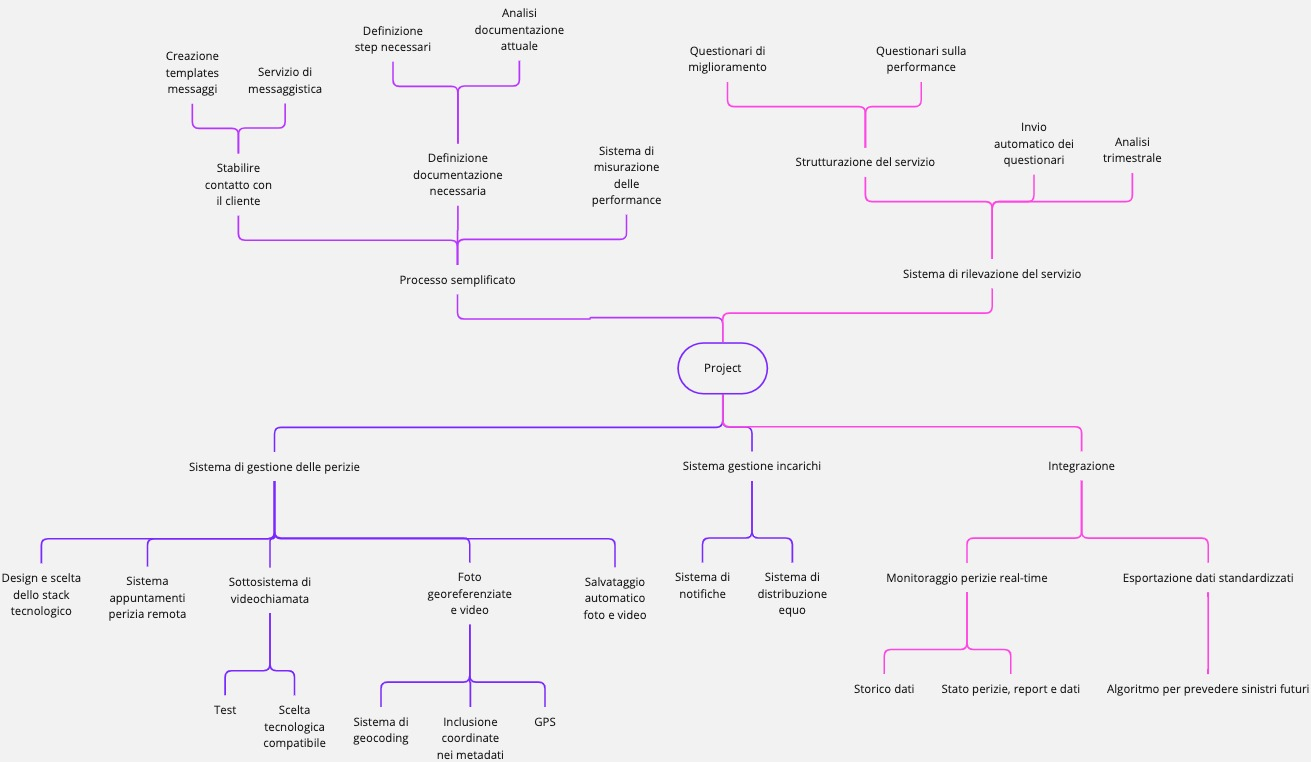
\includegraphics[height=1.0\textwidth,width=1.4\textwidth,angle=-90,origin=c]{img/RBS_map.jpg}
    \caption{Mappa dell'RBS}
    \label{fig:rbs_map}
\end{figure}

\clearpage

\section{Terzo project scoping meeting}
Nel terzo incontro di project scoping, sono stati coinvolti il project manager insieme a un esperto del dominio dell’azienda committente,
oltre all’intero team esecutivo. L'obiettivo principale era confermare la Requirement Breakdown Structure (RBS) e definire il modello di ciclo di vita del progetto (PMLC) da adottare.

\subsection{Modello PMLC}
La decisione di adottare una metodologia Agile all'interno del Project Management Life Cycle (PMLC) per questo progetto è stata basata su una serie di considerazioni strategiche e operazionali. L'approccio Agile è stato scelto per affrontare specifiche esigenze del progetto e per massimizzare l'efficienza nello sviluppo del sistema. 

\subsubsection{Motivazioni della scelta}
\begin{enumerate}
    \item \textbf{Coinvolgimento continuo degli stakeholder}: La metodologia Agile promuove una comunicazione costante e una collaborazione attiva con gli stakeholder migliorando così l'aspetto motivazionale e ottenendo un costante feedback sul lavoro svolto;
    \item \textbf{Coinvolgimento del team di sviluppo}: Coinvolgere il team nei processi permette di far prendere confidenza col dominio, e di anticipare possibili cambiamenti (\textit{Anticipation of Change});
    \item \textbf{Requisiti possibilmente instabili}: In questo contesto, i requisiti possono evolvere rapidamente a causa delle direttive delle compagnie, ma anche a causa delle indecisioni del cliente (studio peritale). L'agile, con i suoi principi di risposta al cambiamento, consente al team di adattarsi in modo flessibile a nuovi requisiti senza dover riprogettare l'intero processo;
    \item \textbf{Consegne incrementali}: La natura iterativa dello sviluppo Agile consente la realizzazione di funzionalità incrementali e il rilascio tempestivo di prodotti intermedi. Questo approccio è particolarmente vantaggioso per questo progetto, in cui è possibile fornire valore ai clienti attraverso funzionalità parziali già durante il processo di sviluppo;
    \item \textbf{Gestione efficace dei rischi}: La metodologia Agile facilita l'identificazione e la gestione tempestiva dei rischi. Attraverso la pianificazione di sprint e la regolare revisione dei risultati ottenuti, il team può rapidamente adattarsi a eventuali sfide o cambiamenti nelle condizioni di progetto;
    \item \textbf{Focus sulla qualità e test continuo}: La pratica dell'agile di integrare il controllo della qualità e i test durante il ciclo di sviluppo favorisce la creazione di un prodotto finale più robusto e di alta qualità. Questo è particolarmente rilevante per questo progetto, dove la precisione e l'affidabilità delle informazioni sono essenziali per il corretto funzionamento del sistema.
\end{enumerate}


\chapter{Planning}

La pianificazione costituisce una fase cruciale nel ciclo di vita della gestione del progetto. È essenziale sostenerla all'inizio del progetto, come suggerisce la ``pain curve'' di Wysocki, al fine di evitare e prevenire difficoltà future. Tale fase è fondamentale poiché permette di delineare gli eventi successivi, riducendo l'incertezza, comprendendo meglio le esigenze del cliente e stabilendo i compiti di ciascun membro del team.\\
Al fine di seguire una buona pratica, è stato deciso di utilizzare Trello come strumento di supporto alla pianificazione, rispetto alla tradizionale lavagna con gli ``sticky notes''. Trello consente di organizzare le attività pianificate, visualizzando quelle già completate, quelle in corso e quelle ancora da avviare.

\section{Durata prevista e partecipanti}
Il progetto è stato classificato come di dimensioni medio-grandi, con una durata massima di pianificazione fissata a 3 giorni. È tuttavia prevista la possibilità di un'estensione di 1 giorno nel caso si verifichino problemi organizzativi o altre circostanze eccezionali. I partecipanti alle riunioni pianificate per questa fase includono::
\begin{itemize}
    \item 1 project manager
    \item Core project team
    \item Client rappresentative
    \item 1 tecnografo
\end{itemize}

Le riunioni sono state programmate in una sala dedicata ai meeting, ma sono state organizzate anche in modalità telematica qualora non fosse possibile svolgerle in presenza a causa della distanza tra i membri del team.

\section{Primo Joint Project Planning Session}

Durante la prima sessione congiunta di pianificazione del progetto, è stata effettuata una sintesi delle discussioni precedenti, focalizzandosi sui documenti creati e sui suggerimenti forniti dagli esperti del dominio. L'obiettivo principale di questa sessione è stato la creazione della ``Work Breakdown Structure'' (WBS), suddividendo il progetto in attività specifiche. Successivamente, le attività sono state priorizzate e sono state definite le dipendenze tra di esse. Il project manager ha adottato il ``Team Approach'', coinvolgendo tutto il team nell'individuazione delle attività principali e nella definizione delle relative dipendenze.

\section{Work Breakdown Structure}
Il team ha delineato la seguente Work Breakdown Structure, riportata di seguito.

\subsubsection{Goal}

Il goal principale di questo progetto è creare un sistema efficiente per la gestione delle perizie di sinistri minori, consentendo ai periti di operare in modo rapido e preciso da remoto, migliorando così i margini di profitto e garantendo un servizio di alta qualità alle compagnie assicurative.

\subsubsection{Requirements}

A partire dal goal principale del progetto, sono stati individuati diversi requisiti.
Di seguito sono elencati i requisiti e il colore indica il livello di priorità assegnatogli come descritto in \ref{prioritizzazione}:
\begin{enumerate}
    \item Processo semplificato;
    \begin{enumerate}
        \item Stabilire contatto con il cliente
        \begin{enumerate}
            \item Creazione templates messaggi
            \begin{enumerate}
                \item \textcolor{blue}{Definizione contenuto messaggi standardizzati in formato HTML}
                \item \textcolor{blue}{Formattazione per diverse piattaforme (email, SMS)}
                \item \textcolor{blue}{Revisione e approvazione}
            \end{enumerate}
            \item Servizio di messaggistica
            \begin{enumerate}
                \item \textcolor{blue}{Selezione piattaforma (Skebby, Twilio, SendGrid, Firebase)}
                \item \textcolor{blue}{Configurazione delle API di invio}
                \item \textcolor{blue}{Test di integrazione}
            \end{enumerate}
            \item Creazione front-end (UI e UX)
            \begin{enumerate}
                \item \textcolor{blue}{Definizione contenuto testo standardizzato}
                \item \textcolor{blue}{Creazione mockup e formattazione per diverse piattaforme mobile (smartphone, tablet)}
                \item \textcolor{blue}{Revisione e approvazione interna}
                \item \textcolor{orange}{Revisione e approvazione tramite focus group}
                \item \textcolor{blue}{Implementazione interfaccia grafica}
            \end{enumerate}
        \end{enumerate}
        \item Definizione documentazione necessaria
        \begin{enumerate}
            \item Analisi documentazione attuale
            \begin{enumerate}
                \item \textcolor{blue}{Raccolta documentazione esistente in un ambiente condiviso}
                \item \textcolor{blue}{Revisione e valutazione}
                \item \textcolor{blue}{Identificazione bottleneck e aree di miglioramento}
            \end{enumerate}
            \item Definizione step necessari
            \begin{enumerate}
                \item \textcolor{blue}{Identificazione passaggi critici con diagrammi di flusso}
                \item \textcolor{blue}{Ottimizzazione flusso di lavoro utilizzando metodologie standard}
                \item \textcolor{blue}{Creazione processo semplificato con rappresentazione a flusso}
            \end{enumerate}
        \end{enumerate}
        \item Sistema di misurazione delle performance
        \begin{enumerate}
            \item \textcolor{teal}{Definizione metriche di base (KPI)}
            \item \textcolor{teal}{Implementazione strumenti di analisi in base alle metriche scelte (risposta, apertura, ...)}
            \item \textcolor{teal}{Generazione di report statici automatizzati}
            \end{enumerate}
    \end{enumerate}
    \item Sistema di rilevazione qualità del servizio
    \begin{enumerate}
        \item Strutturazione dei questionari
        \begin{enumerate}
            \item \textcolor{blue}{Progettazione questionari performance (Google Forms)} 
            \item \textcolor{teal}{Progettazione questionari feedback (Google Forms)} 
            \item \textcolor{orange}{Revisione e approvazione tramite focus group}
        \end{enumerate}
        \item Invio automatico dei questionari
        \begin{enumerate}
            \item \textcolor{teal}{Configurazione del sistema di invio tramite integrazione API (Mail Server)}
            \item \textcolor{teal}{Test di operatività del sistema di invio}
        \end{enumerate}
        \item Analisi trimestrale
        \begin{enumerate}
            \item \textcolor{orange}{Analisi dati utilizzando strumenti di data analysis (Python)}
            \item \textcolor{teal}{Redazione report statici con visualizzazione dati}
            \item \textcolor{blue}{Identificazione azioni correttive}
        \end{enumerate}
    \end{enumerate}
    \item Sistema di gestione delle perizie
    \begin{enumerate}
        \item Design e scelta dello stack tecnologico
        \begin{enumerate}
            \item \textcolor{blue}{Progettazione architettura con diagrammi UML}
            \item \textcolor{blue}{Analisi opzioni disponibili (frameworks, databases)}
            \item \textcolor{blue}{Valutazione e verifica stack tecnologico}
        \end{enumerate}
        \item Sistema appuntamenti perizia remota
        \begin{enumerate}
            \item \textcolor{teal}{Implementazione sistema con calendari integrati}
            \item \textcolor{blue}{Test operatività con casi d'uso reali}
        \end{enumerate}
        \item Sottosistema di videochiamata
        \begin{enumerate}
            \item \textcolor{blue}{Scelta e implementazione tecnologia compatibile (WebRTC)}
            \item Test di operatività del sistema
            \begin{enumerate}
                \item \textcolor{blue}{Pianificazione test su diversi principali dispositivi e reti}
                \item \textcolor{orange}{Esecuzione test con scenari di utilizzo variabili}
                \item \textcolor{blue}{Analisi risultati}
            \end{enumerate}
        \end{enumerate}
        \item Progettazione front-end
        \begin{enumerate}
            \item \textcolor{blue}{Definizione contenuto testo standardizzato}
            \item \textcolor{blue}{Creazione mockup e formattazione per piattaforma desktop}
            \item \textcolor{blue}{Revisione e approvazione interna}
            \item \textcolor{orange}{Revisione e approvazione tramite focus group}
            \item \textcolor{blue}{Implementazione interfaccia grafica}
        \end{enumerate}  
        \item Foto e video georeferenziati
        \begin{enumerate}
            \item Sistema di geocoding
            \begin{enumerate}
                \item \textcolor{blue}{Selezione servizio (Google Maps API, OpenStreetMap)}
                \item \textcolor{blue}{Implementazione servizio con chiamate API}
                \item \textcolor{teal}{Test operatività con dati di esempio}
            \end{enumerate}
            \item Inclusione coordinate nei metadati
            \begin{enumerate}
                \item \textcolor{blue}{Definizione formato (EXIF, GeoJSON)}
                \item \textcolor{blue}{Implementazione}
            \end{enumerate}
            \item GPS
            \begin{enumerate}
                \item \textcolor{blue}{Implementazione collegamento con librerie native}
                \item \textcolor{orange}{Test funzionalità in diverse condizioni ambientali}
            \end{enumerate}
        \end{enumerate}
        \item Salvataggio automatico foto e video
        \begin{enumerate}
            \item \textcolor{teal}{Implementazione del meccanismo di salvataggio automatico con servizi di cloud storage (AWS S3, Google Cloud Storage)}
            \item \textcolor{orange}{Test operatività e simulazioni di carico}
        \end{enumerate}
    \end{enumerate}
    \item Sistema gestione incarichi
    \begin{enumerate}
        \item Sistema di notifiche
        \begin{enumerate}
            \item \textcolor{blue}{Definizione tipologie (Email, SMS)}
            \item \textcolor{teal}{Implementazione infrastruttura}
        \end{enumerate}
        \item Sistema di distribuzione equo
        \begin{enumerate}
            \item \textcolor{teal}{Definizione metriche di assegnamento (carico di lavoro, competenze, disponibilità)}
            \item \textcolor{orange}{Sviluppo dell'algoritmo con tecniche di machine learning (k-means clustering, decision trees)}
            \item \textcolor{orange}{Test operatività dell'algoritmo con dataset realistici (se disponibile storico)}
        \end{enumerate}
    \end{enumerate}
    \item Integrazione
    \begin{enumerate}
        \item Monitoraggio perizie real-time
        \begin{enumerate}
            \item \textcolor{teal}{Storico dati con database NoSQL (MongoDB)}
            \item \textcolor{teal}{Stato perizie, report e dati con l'utilizzo di API}
        \end{enumerate}
        \item Export dati standardizzati
        \begin{enumerate}
            \item \textcolor{teal}{Implementazione meccanismo di esportazione (JSON, XML, YAML, CSV)}
            \item Algoritmo per prevedere sinistri futuri con tecniche machine learning
            \begin{enumerate}
                \item \textcolor{red}{Raccolta e analisi dei dati storici}
                \item \textcolor{red}{Sviluppo dell'algoritmo predittivo (Scikit-learn, TensorFlow)}
                \item \textcolor{red}{Test e validazione algoritmo con dataset di test e tecniche di cross-validation}
            \end{enumerate}
        \end{enumerate}
    \end{enumerate}
\end{enumerate}

\subsection{Prioritizzazione dei requisiti}
\label{prioritizzazione}
In seguito viene stilata una classificazione delle priorità delle attività da effettuare secondo il metodo \textbf{MoSCoW} (\textit{``Must, Should, Could, Won’t have''}), in cui l'aiuto del committente è fondamentale.

Questa classificazione sarà poi d'aiuto per la gestione generale di tali attività.

\begin{itemize}
    \item \textcolor{blue}{\textbf{Must}}: requisiti che \textbf{devono essere soddisfatti} nella soluzione finale per considerare il progetto concluso con successo;
    \item \textcolor{teal}{\textbf{Should}}: requisiti che \textbf{dovrebbero essere inclusi} nella soluzione se è possibile. Solitamente corrispondono a quei requisiti critici che in caso di necessità possono essere sostituiti con dei requisiti alternativi;
    \item \textcolor{orange}{\textbf{Could}}: requisiti che \textbf{potrebbero essere inclusi} nella soluzione ma non sono necessari. Questi requisiti saranno considerati solo se il tempo e le risorse lo permettono;
    \item \textcolor{red}{\textbf{Won’t have}}: requisiti che \textbf{sarebbero da includere} nella soluzione, ma gli stakeholders hanno acconsentito a rinviare l'implementazione in una futura release.
\end{itemize}

\section{Seconda Joint Project Planning Session}

Durante la seconda sessione congiunta di pianificazione del progetto, è stata programmata la condivisione del piano con il committente per ottenere feedback sul lavoro svolto e sulle decisioni prese. I task individuati nella prima riunione sono stati confermati, e si è proceduto alla stima delle risorse e dei tempi necessari per ogni attività. In questa fase, solo il team di lavoro interno ha partecipato attivamente.

\subsection{Stima delle risorse}

Di seguito sono riportate le stime delle risorse umane necessarie per il progetto:
\begin{itemize}
    \item \textbf{Project Manager}: è il coordinatore del progetto, responsabile della pianificazione, esecuzione e controllo delle attività. Si occupa di comunicare con gli stakeholder e gestire i rischi, garantendo che il progetto sia completato nei tempi e nei budget stabiliti;

    \item \textbf{Senior Engineering team}: formato da esperti con competenze tecniche avanzate. Sono responsabili delle soluzioni complesse del progetto e del relativo design, guidano il team per tutta la durata;
    \begin{itemize}
        \item \textbf{Full Stack Engineer}: Si occupa dello sviluppo a 360º dell'applicativo, dal frontend al backend;
        \item \textbf{DevOps and QA Engineer}: Responsabile della gestione e ottimizzazione delle pratiche DevOps, che spaziano dal testing al delivery. Si occupa del testing del software, garantendo che ogni componente soddisfi i requisiti di qualità.
    \end{itemize}

    \item \textbf{Junior Engineering team}: composto da membri meno esperti, si occupa dell'implementazione di componenti più semplici del progetto, con l'obiettivo di acquisire competenze e crescere professionalmente;

    \item \textbf{Business Analyst}: Si dedica alla raccolta e analisi dei requisiti seguendo un'ottica di business assicurando che le esigenze degli stakeholder siano comprese e documentate correttamente. Facilita la comunicazione tra il team tecnico e gli stakeholder per garantire che le soluzioni sviluppate soddisfino le aspettative del cliente, mira a una early win;
    
    \item \textbf{UX/UI Designer}: progetta l'interfaccia utente del sistema, creando mockup e prototipi per assicurare un'esperienza ottimale. Si assicura che il design sia intuitivo, efficiente e conforme alle esigenze degli utenti finali.
    
\end{itemize}

\subsection{Stima dei tempi}

Per la stima dei tempi è stato adottato un metodo di stima ``consensus-based'', in particolare la tecnica Delphi. In questa procedura, l'unità di misura scelta è stata l'ora/uomo, al fine di garantire chiarezza e conformità nella valutazione temporale.
Per ciascuna foglia della WBS è stato specificato il numero di ore/uomo necessarie, e ogni elemento di dettaglio della WBS sarà convertito in una potenziale attività per lo sviluppatore designato.
Inoltre, per garantire una comprensione precisa di cosa comporta il completamento di una singola attività, è stato deciso di stabilire formalmente le Definition of Done (DoD), ovvero i criteri specifici che determinano quando una task può considerarsi conclusa.

\subsubsection{Definition of Done}
Un'attività per dichiarsi conclusa richiede che i seguenti punti siano stati effettuati:
\begin{itemize}
    \item Sviluppo del core della task;
    \item Sviluppo di un numero adeguato di test;
    \item Code Review da parte di almeno un altro membro del team;
    \item Verifica da parte del QA engineer per le task che lo richiedono (test non automatizzabili);
    \item Documentazione relativa alla nuova contribuzione, con eventuale revisione di quella già esistente.
\end{itemize}

\subsubsection{Tempi}

\begin{enumerate}
    \item Processo semplificato
    \begin{enumerate}
        \item Stabilire contatto con il cliente
        \begin{enumerate}
            \item Creazione templates messaggi
            \begin{table}[h]
                \centering
                \begin{tabularx}{0.8\textwidth}{ | m{8cm} | >{\centering\arraybackslash}X | }
                    \hline
                    Definizione contenuto messaggi standardizzati in formato HTML & 4.5 \\
                    \hline
                    Formattazione per diverse piattaforme & 3.5 \\
                    \hline
                    Revisione e approvazione & 2 \\
                    \hline
                \end{tabularx}
            \end{table}
            \item Servizio di messaggistica
            \begin{table}[h]
                \centering
                \begin{tabularx}{0.8\textwidth}{ | m{8cm} | >{\centering\arraybackslash}X | }
                    \hline
                     Selezione piattaforma (Skebby, Twilio, SendGrid, Firebase) & 4 \\
                    \hline
                    Configurazione delle API di invio & 7 \\
                    \hline
                    Test di integrazione & 3.5 \\
                    \hline
                \end{tabularx}
            \end{table}
            
            \item Creazione front-end (UI e UX)
            \begin{table}[!htp]
                \centering
                \begin{tabularx}{0.8\textwidth}{ | m{8cm} | >{\centering\arraybackslash}X | }
                    \hline
                    Definizione contenuto testo standardizzato & 6.5 \\
                    \hline
                    Creazione mockup e formattazione per diverse piattaforme mobile (smartphone, tablet) & 16 \\
                    \hline
                    Revisione e approvazione interna & 3 \\
                    \hline
                    Revisione e approvazione tramite focus group & 8 \\
                    \hline
                    Implementazione interfaccia grafica & 24\\
                    \hline
                \end{tabularx}
            \end{table}
        \end{enumerate}
        \clearpage
        \item Definizione documentazione necessaria
        \begin{enumerate}
            \item Analisi documentazione attuale
            \begin{table}[h]
                \centering
                \begin{tabularx}{0.8\textwidth}{ | m{8cm} | >{\centering\arraybackslash}X | }
                    \hline
                    Raccolta documentazione esistente in un ambiente condiviso & 2.5 \\
                    \hline
                    Revisione e valutazione & 4 \\
                    \hline
                    Identificazione bottleneck e aree di miglioramento & 14 \\
                    \hline
                \end{tabularx}
            \end{table}
            \item Definizione step necessari
            \begin{table}[h]
                \centering
                \begin{tabularx}{0.8\textwidth}{ | m{8cm} | >{\centering\arraybackslash}X | }
                    \hline
                     Identificazione passaggi critici con diagrammi di flusso & 10 \\
                    \hline
                    Ottimizzazione flusso di lavoro utilizzando metodologie standard & 12 \\
                    \hline
                    Creazione processo semplificato con rappresentazione a flusso & 7 \\
                    \hline
                \end{tabularx}
            \end{table}
        \end{enumerate}
        \item Sistema di misurazione delle performance
            \begin{table}[h]
                \centering
                \begin{tabularx}{0.8\textwidth}{ | m{8cm} | >{\centering\arraybackslash}X | }
                    \hline
                    Definizione metriche di base (KPI) & 8 \\
                    \hline
                    Implementazione strumenti di analisi in base alle metriche scelte (risposta, apertura, ecc...) & 24 \\
                    \hline
                    Generazione di report statici automatizzati & 17 \\
                    \hline
                \end{tabularx}
            \end{table}
    \end{enumerate}
    \item Sistema di rilevazione qualità del servizio
    \begin{enumerate}
        \item Strutturazione dei questionari
            \begin{table}[!h]
                \centering
                \begin{tabularx}{0.8\textwidth}{ | m{8cm} | >{\centering\arraybackslash}X | }
                    \hline
                    Progettazione questionari performance (Google Forms) & 8 \\
                    \hline
                    Progettazione questionari feedback (Google Forms) & 4.5 \\
                    \hline
                    Revisione e approvazione tramite focus group & 7 \\
                    \hline
                \end{tabularx}
            \end{table}
        \clearpage
        \item Invio automatico dei questionari
            \begin{table}[h]
                \centering
                \begin{tabularx}{0.8\textwidth}{ | m{8cm} | >{\centering\arraybackslash}X | }
                    \hline
                    Configurazione del sistema di invio tramite integrazione API (Mail Server) & 18 \\
                    \hline
                    Test di operatività del sistema di invio & 4 \\
                    \hline
                \end{tabularx}
            \end{table}
        \item Analisi trimestrale
        \begin{table}[h]
                \centering
                \begin{tabularx}{0.8\textwidth}{ | m{8cm} | >{\centering\arraybackslash}X | }
                    \hline
                    Analisi dati utilizzando strumenti di data analysis (Python) & 14 \\
                    \hline
                    Redazione report statici con visualizzazione dati & 16 \\
                    \hline
                    Identificazione azioni correttive & 8\\
                    \hline
                \end{tabularx}
            \end{table}
    \end{enumerate}
    \item Sistema di gestione delle perizie
    \begin{enumerate}
        \item Design e scelta dello stack tecnologico
        \begin{table}[h]
            \centering
            \begin{tabularx}{0.8\textwidth}{ | m{8cm} | >{\centering\arraybackslash}X | }
                \hline
                Progettazione architettura con diagrammi UML & 36 \\
                \hline
                Analisi opzioni disponibili (frameworks, databases) & 6 \\
                \hline
                Valutazione e verifica stack tecnologico & 4 \\
                \hline
            \end{tabularx}
        \end{table}
        \item Sistema appuntamenti perizia remota
        \begin{table}[!h]
            \centering
            \begin{tabularx}{0.8\textwidth}{ | m{8cm} | >{\centering\arraybackslash}X | }
                \hline
                Implementazione sistema con calendari integrati & 32 \\
                \hline
                Test operatività con casi d'uso reali & 4 \\
                \hline
            \end{tabularx}
        \end{table}
        \item Sottosistema di videochiamata
        \begin{table}[!h]
            \centering
            \begin{tabularx}{0.8\textwidth}{ | m{8cm} | >{\centering\arraybackslash}X | }
                \hline
                Scelta e implementazione tecnologia compatibile (WebRTC) & 32 \\
                \hline
            \end{tabularx}
        \end{table}
        \clearpage
        \begin{enumerate}
            \item Test di operatività del sistema
            \begin{table}[h]
                \centering
                \begin{tabularx}{0.8\textwidth}{ | m{8cm} | >{\centering\arraybackslash}X | }
                    \hline
                    Pianificazione test su diversi principali dispositivi e reti & 5 \\
                    \hline
                    Esecuzione test con scenari di utilizzo variabili & 3.5 \\
                    \hline
                    Analisi risultati & 2 \\
                    \hline
                \end{tabularx}
            \end{table}
        \end{enumerate}
        \item Progettazione front-end
        \begin{table}[h]
            \centering
            \begin{tabularx}{0.8\textwidth}{ | m{8cm} | >{\centering\arraybackslash}X | }
                \hline
                Definizione contenuto testo standardizzato & 8 \\
                \hline
                Creazione mockup e formattazione per piattaforma desktop & 32 \\
                \hline
                Revisione e approvazione interna & 4 \\
                \hline
                Revisione e approvazione tramite focus group & 8 \\
                \hline
                Implementazione interfaccia grafica & 40\\
                \hline
            \end{tabularx}
        \end{table}
        \item Foto e video georeferenziati
        \begin{enumerate}
            \item Sistema di geocoding
            \begin{table}[!h]
                \centering
                \begin{tabularx}{0.8\textwidth}{ | m{8cm} | >{\centering\arraybackslash}X | }
                    \hline
                    Selezione servizio & 2 \\
                    \hline
                    Implementazione servizio con chiamate API & 12 \\
                    \hline
                    Test operatività con dati di esempio & 3 \\
                    \hline
                \end{tabularx}
            \end{table}
            \item Inclusione coordinate nei metadati
            \begin{table}[!h]
                \centering
                \begin{tabularx}{0.8\textwidth}{ | m{8cm} | >{\centering\arraybackslash}X | }
                    \hline
                    Definizione formato & 1 \\
                    \hline
                    Implementazione & 3 \\
                    \hline
                \end{tabularx}
            \end{table}
            \item GPS
            \begin{table}[!h]
                \centering
                \begin{tabularx}{0.8\textwidth}{ | m{8cm} | >{\centering\arraybackslash}X | }
                    \hline
                    Implementazione collegamento con librerie native & 2 \\
                    \hline
                    Test funzionalità in diverse condizioni ambientali & 2 \\
                    \hline
                \end{tabularx}
            \end{table}
            \clearpage
        \end{enumerate}
        \item Salvataggio automatico foto e video
        \begin{table}[h]
            \centering
            \begin{tabularx}{0.8\textwidth}{ | m{8cm} | >{\centering\arraybackslash}X | }
                \hline
                Implementazione del meccanismo di salvataggio automatico con servizi di cloud storage & 24 \\
                \hline
                Test operatività e simulazioni di carico & 3 \\
                \hline
            \end{tabularx}
        \end{table}
    \end{enumerate}
    \item Sistema gestione incarichi
    \begin{enumerate}
        \item Sistema di notifiche
        \begin{table}[!h]
            \centering
            \begin{tabularx}{0.8\textwidth}{ | m{8cm} | >{\centering\arraybackslash}X | }
                \hline
                Definizione tipologie & 2.5 \\
                \hline
                Implementazione infrastruttura & 12 \\
                \hline
            \end{tabularx}
        \end{table}
        \item Sistema di distribuzione equo
        \begin{table}[!h]
            \centering
            \begin{tabularx}{0.8\textwidth}{ | m{8cm} | >{\centering\arraybackslash}X | }
                \hline
                Definizione metriche di assegnamento & 5 \\
                \hline
                Sviluppo dell'algoritmo con tecniche di machine learning & 30 \\
                \hline
                Test operatività dell'algoritmo con dataset realistici & 8 \\
                \hline
            \end{tabularx}
        \end{table}
    \end{enumerate}
    \item Integrazione
    \begin{enumerate}
        \item Monitoraggio perizie real-time
        \begin{table}[!h]
            \centering
            \begin{tabularx}{0.8\textwidth}{ | m{8cm} | >{\centering\arraybackslash}X | }
                \hline
                Storico dati con database NoSQL & 12 \\
                \hline
                Stato perizie, report e dati con l'utilizzo di API & 32 \\
                \hline
            \end{tabularx}
        \end{table}
        \item Export dati standardizzati
        \begin{enumerate}
            \begin{table}[!h]
                \centering
                \begin{tabularx}{0.8\textwidth}{ | m{8cm} | >{\centering\arraybackslash}X | }
                    \hline
                    Implementazione meccanismo di esportazione (JSON, XML, YAML, CSV) & 8 \\
                    \hline
                \end{tabularx}
            \end{table}
            \clearpage
            \item Algoritmo per prevedere sinistri futuri con tecniche machine learning
            \begin{table}[h]
                \centering
                \begin{tabularx}{0.8\textwidth}{ | m{8cm} | >{\centering\arraybackslash}X | }
                    \hline
                    Raccolta e analisi dei dati storici & 5 \\
                    \hline
                    Sviluppo dell'algoritmo predittivo & 40 \\
                    \hline
                    Test e validazione algoritmo con dataset di test e tecniche di cross-validation & 20 \\
                    \hline
                \end{tabularx}
            \end{table}
        \end{enumerate}
    \end{enumerate}
\end{enumerate}


\subsection{Stima dei costi}

La pianificazione del progetto deve considerare attentamente il tipo di contratto stipulato tra l'azienda esecutrice e il committente. A tal fine, è stato valutato e scelto di adottare un approccio misto, combinando un contratto a corpo e a misura, come descritto successivamente. Il modello si basa sul calcolo del corrispettivo in base alle risorse impiegate nel processo produttivo, considerando sia il tempo sia le spese associate. Inoltre, è previsto l'utilizzo di una scope bank per gestire e monitorare l'evoluzione degli obiettivi e dei requisiti del progetto, assicurando una corretta allocazione delle risorse. Il cash flow management sarà cruciale per garantire un flusso finanziario stabile durante l'intera durata del progetto, ottimizzando la disponibilità dei fondi per le necessità operative e minimizzando il rischio finanziario. 
Le aziende hanno concordato su questa modalità contrattuale, con la clausola di prezzo massimo di 50.000 € per i requisiti denotati come ``Must'' e ``Should''. In questo caso, il corrispettivo sarà a corpo, fornendo al cliente la sicurezza di quanto spenderà per ottenere un software funzionante. Per i requisiti denotati come ``Could'' e ``Won't Have'', invece, il corrispettivo sarà a misura, consentendo flessibilità e disponibilità per nuove implementazioni. Questa scelta è stata possibile grazie all'esperienza maturata internamente in progetti di video streaming, facilitando la determinazione delle ore e dei giorni/uomo necessari per la parte core del progetto. Per gli sviluppi ``Could'' e ``Won't Have'', le ore necessarie e il costo associato saranno determinati sulla base di tariffe standard per figura professionale. Questa scelta è stata inoltre adottata a causa del vincolo di spesa massima per un software funzionante imposto dal cliente, data la sua situazione a rischio.
Per quanto riguarda invece la gestione del cash flow management si è deciso di procedere a queste condizioni: 
\begin{itemize}
    \item Anticipo: 25\% alla firma del contratto;
    \item Milestone: descritte successivamente; 
    \item Saldo: a chiusura del progetto tenendo in considerazione il sesto quinto sulla base del tempo di consegna.
\end{itemize}

\section{Project Network Diagram}
Di seguito è presente il Gantt Chart \ref{fig:gantt} dove vengono rappresentate le attività definite nella WBS. I colori, invece, indicano i macro obiettivi della WBS.

\begin{figure}[htp]
    \centering    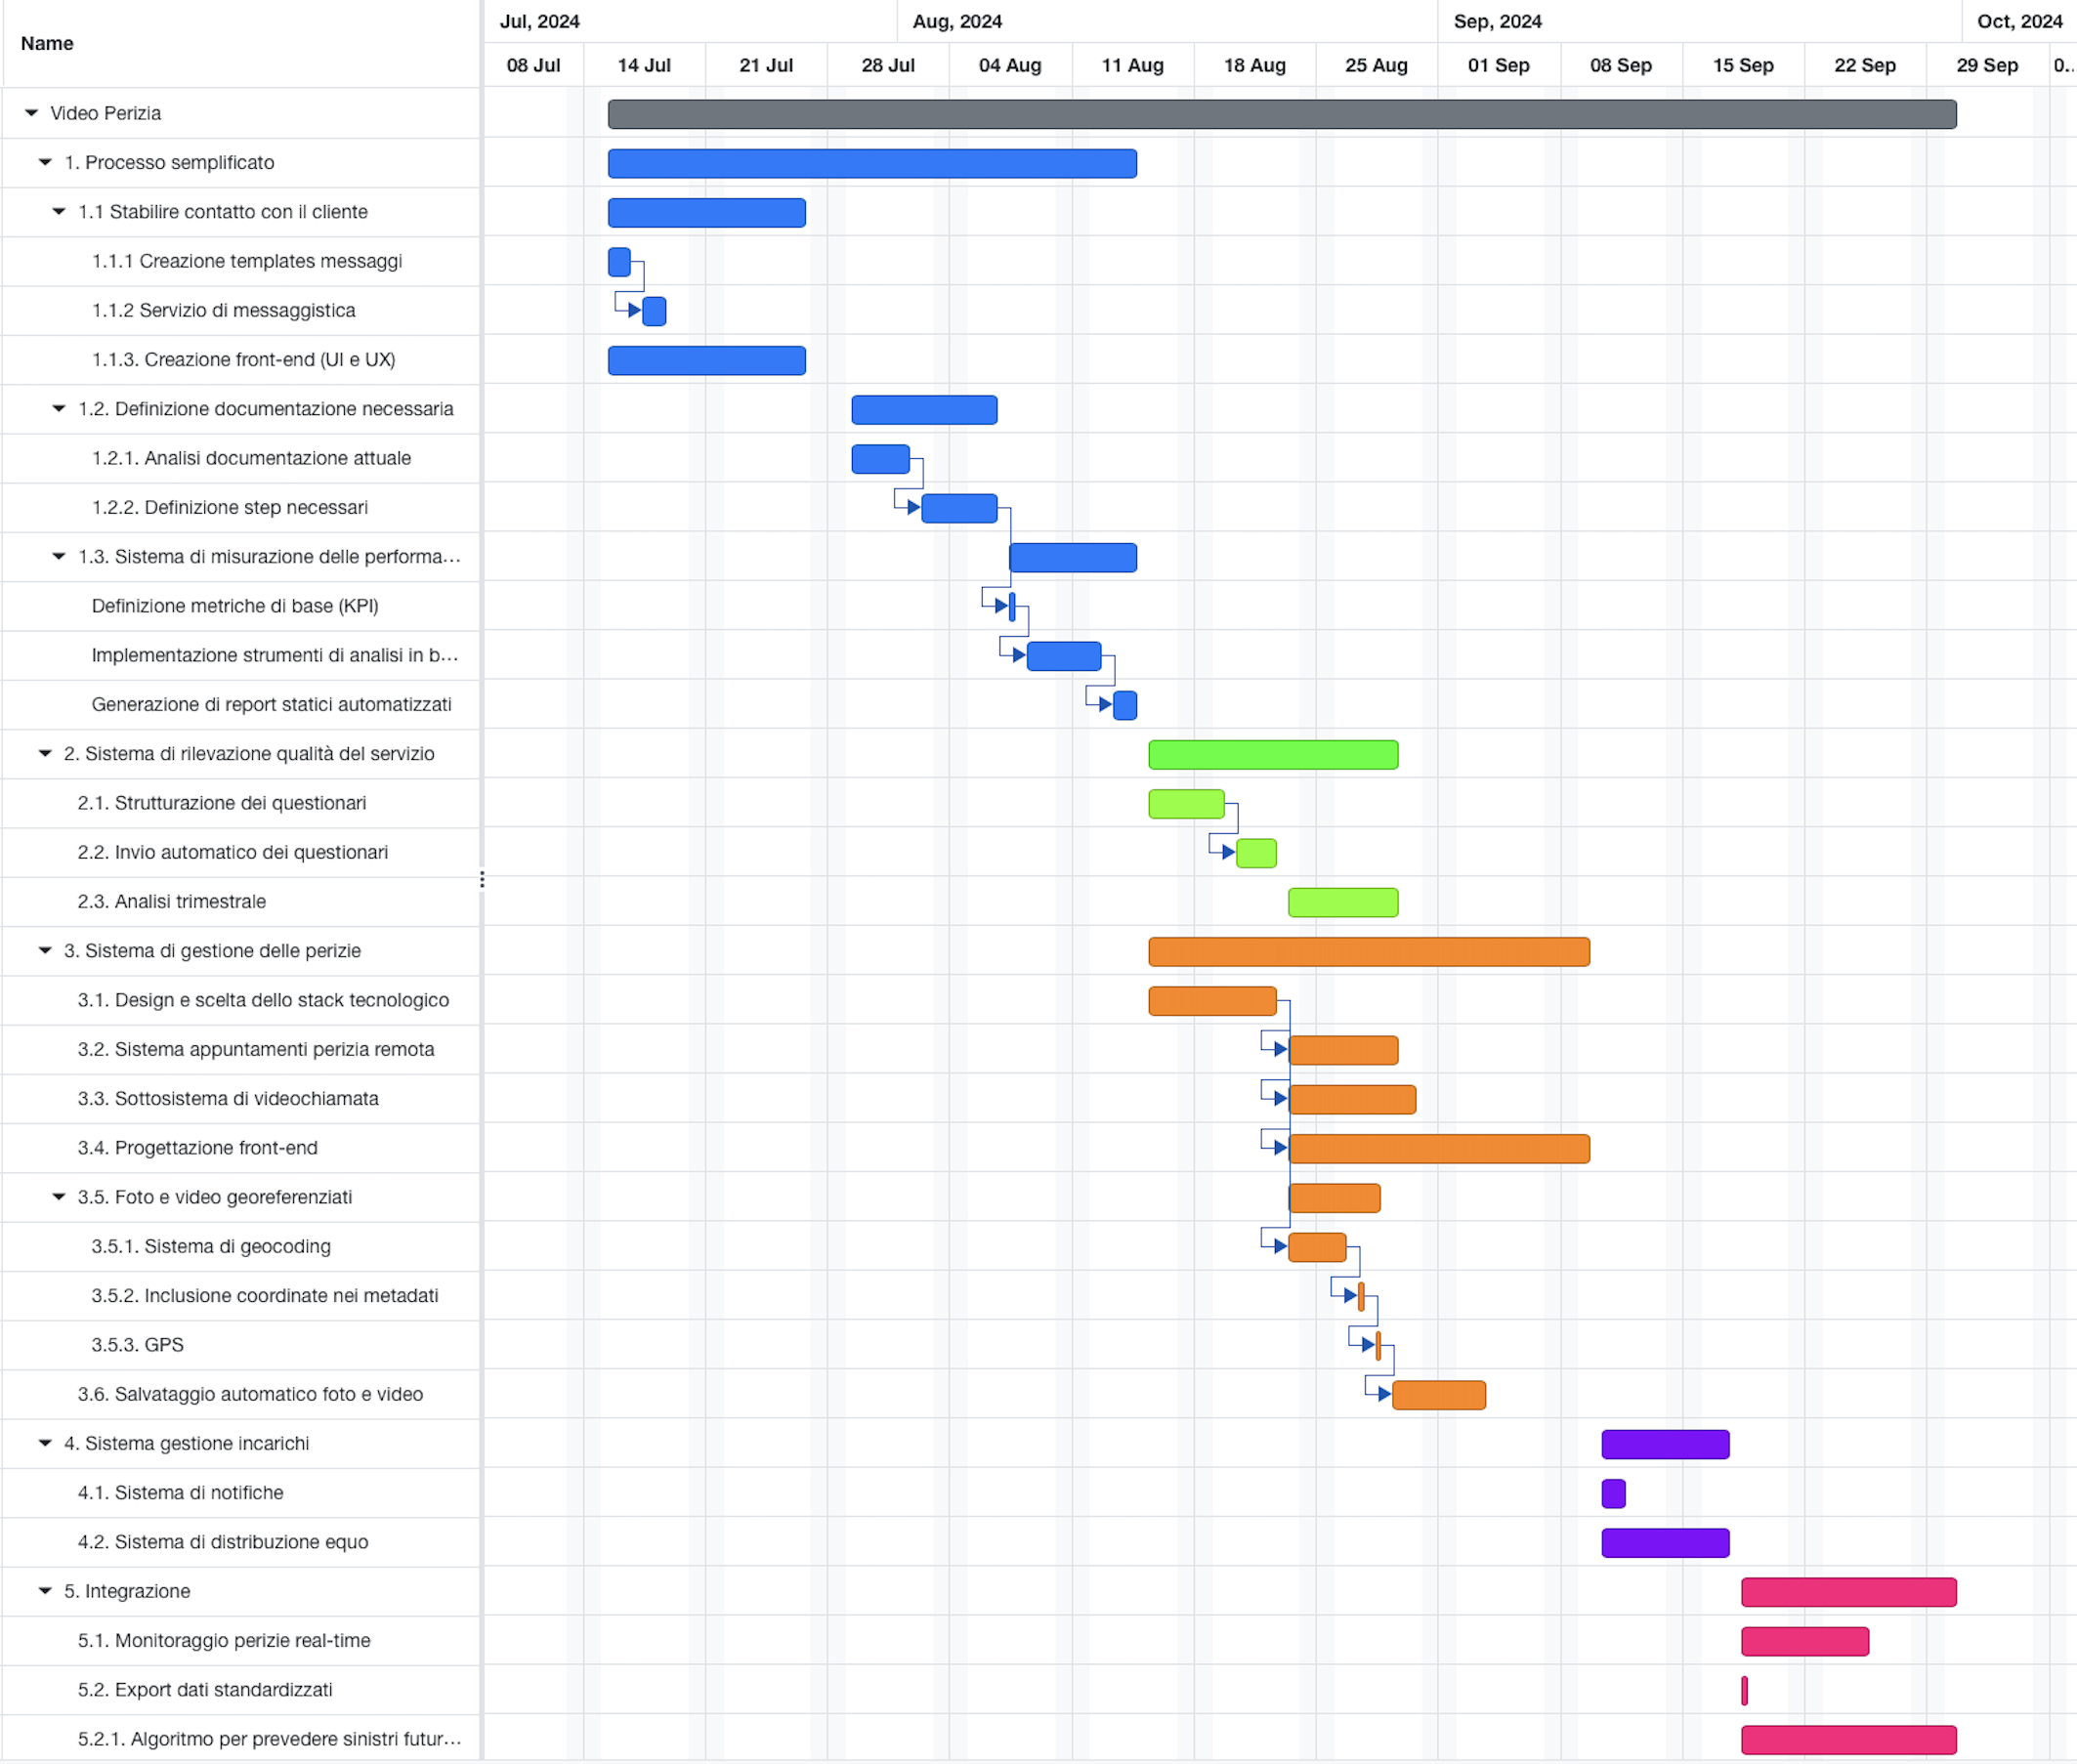
\includegraphics[height=1.0\textwidth,width=1.5\textwidth,angle=-90,origin=c]{img/gantt.png}
    \caption{Gantt}
    \label{fig:gantt}
\end{figure}

\section{Terza Joint Project Planning Session}
Nell'ultima sessione vi partecipano solo i dipendenti dell'azienda esecutrice e riguarda l'ottenimento dell'approvazione da parte di tutti i partecipanti sui contenuti del piano, previa identificazione dei rischi con eventuale piano di mitigazione, ma questa fase è stata affrontata precedentemente, per cui deve solo essere rielaborata.
Il progetto è strutturato in milestone principali, ognuna delle quali verrà completata in un intervallo di 2-3 settimane. Le milestone sono definite come segue:
\begin{enumerate}
    \item Template di messaggi, mockup front-end e documentazione necessaria.
    \item Sistema di misurazione delle performance, questionari, invii automatici e template di report statici.
    \item Sistema di videochiamata, sistema di messaggistica e relativi front-end.
    \item Sistema di geocoding e salvataggio automatico.
    \item Gestione incarichi e sistema di appuntamenti perizie.
    \item Integrazione.
\end{enumerate}

\subsection{Analisi dei rischi}
Durante la fase di scoping del progetto, è stata condotta una prima analisi dei rischi che viene ulteriormente arricchita durante la fase di pianificazione. La gestione del rischio rappresenta una fase cruciale per l'anticipazione di imprevisti durante l'intero ciclo di vita del progetto. È essenziale continuare a identificare potenziali rischi e farlo in modo continuo durante lo sviluppo del progetto, particolarmente ogni volta che si devono prendere decisioni critiche.

Facendo riferimento sempre alla figura \ref{fig:risk}, abbiamo indivuato ulteriori rischi non emersi nella fase iniziale:
\begin{enumerate}
    \item \textbf{Utilizzo intuitivo lato assicurato}: Per quanto riguarda l'utilizzo del servizio lato assicurato è stato specificatamente richiesto un utilizzo adeguato anche per neofiti
    \\
    \textbf{Stima}: Medio (9)
    \\
    \textbf{Possibile mitigazione}: Ridurre al minimo il numero di click per poter entrare in contatto con un perito, rassicurando gli utenti meno tecnologici.
    \item \textbf{Scelta tecnologica}: L'utilizzo di una nuove tecnologie potrebbe comportare un ritardo nella timeline.
    \\
    \textbf{Stima}: Basso (4)
    \\
    \textbf{Possibile mitigazione}: Condurre una valutazione approfondita prima di adottare una nuova tecnologia. Effetturare test per valutare l'efficacia e consultare sviluppatori.
    \item \textbf{Cambiamenti normativi}: Modifiche nei requisiti legali e normativi possono influenzare il progetto.
    \\
    \textbf{Stima}: Medio (4)
    \\
    \textbf{Possibile mitigazione}: Mantenere uno stretto monitoraggio degli sviluppi normativi e adattare il progetto di conseguenza.
\end{enumerate}

\subsection{Project Description Statement}
Il PDS rappresenta una versione estesa del POS e contiene una definizione del progetto più dettagliata, utilizzata dal team per avere una visione comune sul progetto. Inoltre, risulta anche essere un punto di riferimento per eventuali nuovi membri del team.

\subsubsection{Problem/Opportunity}
Lo studio peritale X ha subito un calo del margine di profitto del 35\%. Inizialmente si pensava fosse dovuto a una diminuzione del carico di lavoro, ma si è scoperto che il problema è legato alla mancanza di efficienza dei processi interni, soprattutto per le perizie relative a sinistri minori. Questi sinistri, pur avendo margini di guadagno relativamente bassi, rappresentano una grossa fetta del mercato e garantiscono buone performance alle compagnie assicurative, permettendo di ottenere incarichi più remunerativi.

\subsubsection{Project Goal}
Implementare un sistema innovativo per la gestione delle perizie di sinistri minori presso lo studio peritale X. Questo sistema mira a ottimizzare i processi interni, migliorando l'efficienza, la rapidità e la qualità del servizio offerto alle compagnie assicurative. L'obiettivo principale è aumentare i margini di profitto consentendo ai periti di gestire un volume maggiore di perizie minori in meno tempo, rafforzando la fiducia delle compagnie assicurative. Questo sistema includerà le seguenti caratteristiche:
\begin{enumerate}
    \item \textbf{Automazione dei Processi}: L'introduzione di workflow automatizzati per la gestione delle perizie e relativi incarichi, dalla ricezione del sinistro alla chiusura dell'incarico;
    \item \textbf{Sistema di Gestione degli Incarichi}: Un sistema per l'assegnazione automatica delle perizie ai periti disponibili, basato su criteri predefiniti come il carico di lavoro, le competenze e la disponibilità;
    \item \textbf{Perizie da Remoto}: Integrazione di un sistema di videochiamata sicuro che consenta ai periti di effettuare perizie da remoto attraverso postazioni desktop ben organizzate, ma che al tempo stesso garantisca i requisiti di sicurezza e anti-frode come la localizzazione GPS;
    \item \textbf{Interfaccia Utente Intuitiva}: Un'interfaccia utente user-friendly che guidi i periti attraverso il processo di perizia.
    \item \textbf{Analisi delle Performance}: Un sistema di reportistica che consenta di analizzare le performance del processo di perizia, identificando aree di miglioramento e misurando la soddisfazione del cliente tramite questionari di valutazione, ma che garantisca anche una misurazione delle performance dei periti;
    \item \textbf{Integrazione con Sistemi Esistenti}: Capacità di integrare il nuovo software con i sistemi informatici già in uso presso le compagnie assicurative, garantendo così una transizione fluida e senza interruzioni. Inoltre il sistema dovrà essere aperto a modifiche in caso in cui le compagnie assicurative richiedano specifiche funzionalità di data retrieve (tenendo anche in considerazione le norme vigenti che potranno subire modifiche).
\end{enumerate}

\subsubsection{Project Objectives}
Gli obiettivi sono:
\begin{enumerate}
    \item Creare un processo parallelo al tradizionale per gestire un maggior numero di perizie relative a sinistri minori, eliminando gli step superflui, ottimizzando alcuni già esistenti o creandone di nuove;
    \item Implementare un sistema di gestione che consenta di effettuare perizie da remoto attraverso una piattaforma che permetta il video streaming;
    \item Creare un sistema di gestione degli incarichi per i periti che sia il più fair possibile attraverso metriche predefinite;
    \item Aggiungere nel processo esistente un servizio per valutare la soddisfazione degli utenti e dei periti attraverso la fruizione di questionari;
    \item Fornire alle compagnie assicurative APIs che permetta di consultare lo stato delle perizie gestite in tempo reale.
\end{enumerate}

\subsubsection{Success Criteria}
\begin{itemize}
    \item Recupero del 35\% di perdite entro un anno;
    \item Incremento del margine di profitto del 10\% entro due anni;
    \item Miglioramento della qualità del servizio offerto alle compagnie assicurative e ai clienti;
    \item Incremento del 50\% nella gestione dei sinistri minori entro un anno;
    \item Raggiungimento della competitività di mercato entro un anno.
\end{itemize}

\subsubsection{Assunzioni}
\begin{itemize}
    \item Disponibilità delle infrastrutture necessarie come postazioni desktop, cuffie, microfoni, webcam e una connessione internet stabile;
    \item L'assicurato dispone di una connessione internet sufficientemente veloce.
    \item Il personale dello studio peritale X sarà adeguatamente formato all'utilizzo del nuovo sistema;
    \item Gli ambienti di sviluppo, test e produzione saranno configurati e disponibili per tutte le fasi del progetto;
    \item Il team di sviluppo avrà accesso continuo alla documentazione tecnica e ai requisiti funzionali necessari, disponendo inoltre di un ambiente condiviso per caricare documenti o file che si ritengono necessari o importanti;
    \item Eventuali dipendenze da terze parti, come API esterne o servizi cloud, saranno stabili e disponibili per la durata del progetto;
    \item Le policy aziendali e le normative vigenti in materia di privacy e sicurezza dei dati saranno rispettate durante tutto il ciclo di vita del progetto.
\end{itemize} 

\subsubsection{Rischi}
\begin{itemize}
    \item Potenziale resistenza al cambiamento da parte del personale, che potrebbe rallentare l'adozione del nuovo sistema e ridurre l'efficienza operativa;
    \item Incapacità dello studio peritale di gestire il nuovo carico di lavoro, richiedendo nuove assunzioni o una riorganizzazione interna con costi aggiuntivi;
    \item Necessità di conformarsi ai vincoli di data privacy e sicurezza dei dati personali imposti dalle normative vigenti e dalle compagnie assicurative;
    \item Potenziale incompatibilità del sistema con i sistemi informatici delle compagnie assicurative;
    \item La perizia effettuata da remoto potrebbe non raggiungere l'accuratezza delle perizie tradizionali in presenza;
    \item Possibile inadeguatezza delle infrastrutture esistenti nel supportare il carico operativo del nuovo sistema, richiedendo aggiornamenti hardware o di rete lato studio peritale;
    \item Possibile aumento imprevisto nel volume di perizie senza degradare la qualità del servizio.
\end{itemize}

\subsubsection{Ostacoli}
\begin{itemize}
    \item La creazione di un sistema in grado di eseguire video-perizie comporta una gestione tecnica complessa, che dovrà essere completamente gestita dal team senza che il cliente ne risenta;
    \item Garantire una user experience ottimale per gli utenti finali, sia per i periti che per i clienti, sarà una sfida data la necessità di integrare numerose funzionalità;
    \item Assicurare la compatibilità cross-platform del sistema di video-perizie, garantendo funzionamento fluido su diversi dispositivi, sistemi operativi e browser;
    \item Gestione della latenza e della qualità delle videochiamate, assicurando che il sistema mantenga prestazioni elevate anche in condizioni di connettività internet variabile, da tenere in considerazione durante la scelta del framework di video-streaming.
\end{itemize}


\subsection{Criteri di accettazione}
É buona norma definire in modo chiaro, con la collaborazione del committente, i criteri di accettazione durante la fase di planning. Con essi verrà verificata la chiusura del progetto durante la fase di Closing. A tale scopo, l'elenco dei criteri di accettazione vengono valutati ad ogni milestone. Di seguito sono riportati alcuni criteri di accettazione aggiuntivi per ciascuna delle milestone elencate:
\begin{enumerate}
    \item \textbf{Template di messaggi, mockup front-end e documentazione necessaria}:
    \begin{itemize}
        \item \textbf{Template di messaggi}: I template devono essere conformi ai requisiti di formato e contenuto definiti. Devono essere approvati dal committente e testati per la compatibilità con le piattaforme previste (Email, SMS). Se il cliente riterrà necessario avrà la possibilità di chiedere consulenza legale per i contenuti;
        \item \textbf{Mockup front-end}: I mockup devono rispecchiare i requisiti di design e usabilità concordati. Devono essere approvati dal committente e revisionati in base ai feedback ricevuti;
        \item \textbf{Documentazione necessaria}: La documentazione deve essere completa, chiara e comprensibile, e deve includere tutte le informazioni necessarie per l'utilizzo e la manutenzione del sistema. Deve essere approvata dal committente.
    \end{itemize}
    \item \textbf{Sistema di misurazione delle performance, questionari, invii automatici e template di report statici}:
    \begin{itemize}
        \item \textbf{Sistema di misurazione delle performance}: Le metriche di base devono essere correttamente implementate e verificate attraverso test specifici. I report devono rispecchiare i dati attesi e fornire insight utili;
        \item \textbf{Questionari}: I questionari devono essere completi, con domande chiare e pertinenti. Devono essere approvati dal committente e testati per garantire che vengano raccolte le informazioni desiderate;
        \item \textbf{Invii automatici}: I meccanismi di invio automatico devono funzionare correttamente, rispettando le tempistiche e i criteri di invio definiti;
        \item \textbf{Template di report statici}: I report devono essere generati correttamente secondo i template definiti e devono presentare i dati in modo chiaro e coerente.
    \end{itemize}
    \item \textbf{Sistema di videochiamata, sistema di messaggistica e relativi front-end}:
    \begin{itemize}
        \item \textbf{Sistema di videochiamata}: Il sistema deve supportare videochiamate di qualità e deve funzionare senza interruzioni. Devono essere completati i test su diversi dispositivi e reti;
        \item \textbf{Sistema di messaggistica}: La messaggistica deve essere stabile e sicura, con funzionalità testate e verificate per il corretto invio e ricezione dei messaggi;
        \item \textbf{Front-end}: I front-end per videochiamate e messaggistica devono essere intuitivi e conformi ai requisiti di design. Devono essere approvati dal committente e testati per l'usabilità.
    \end{itemize}
    \item \textbf{Sistema di geocoding e salvataggio automatico}:
    \begin{itemize}
        \item \textbf{Sistema di geocoding}: Il sistema deve fornire risultati di geocoding precisi e deve gestire correttamente le coordinate geografiche;
        \item \textbf{Salvataggio automatico}: Il meccanismo di salvataggio automatico deve essere affidabile, con backup e recupero dei dati testati e verificati.
    \end{itemize}
    \item \textbf{Gestione incarichi e sistema di appuntamenti perizie}:
    \begin{itemize}
        \item \textbf{Gestione incarichi}: Il sistema deve consentire una gestione efficace e trasparente degli incarichi, con funzionalità di assegnazione, monitoraggio e aggiornamento;
        \item \textbf{Sistema di appuntamenti perizie}: Il sistema deve gestire efficacemente gli appuntamenti perizie, con funzionalità di pianificazione, notifiche e integrazione con i calendari.
    \end{itemize}
    \item \textbf{Integrazione}:
    \begin{itemize}
        \item \textbf{Integrazione dei sistemi}: Tutti i sistemi devono essere integrati senza errori, con flussi di dati e comunicazioni testati tra le diverse componenti del sistema;
        \item \textbf{Test di integrazione}: Devono essere completati test di integrazione per verificare la funzionalità complessiva del sistema e la corretta interazione tra i diversi moduli e servizi delle compagnie.
    \end{itemize}
\end{enumerate}


\chapter{Launching and Execution}

La fase di avvio ed esecuzione di un progetto riveste un'importanza fondamentale per tradurre la pianificazione in azione concreta. Durante questo stadio, si procede con la selezione del personale da inserire nel team di progetto, si definiscono le regole operative del gruppo e si facilita la collaborazione all'interno del team, al fine di lavorare in modo efficace e conseguire gli obiettivi prefissati.

\section{Team di sviluppo}
Successivamente alla fase di pianificazione, è stato definito il team di sviluppo, composto da:
\begin{itemize}
    \item 1 Project manager
    \item 2 Senior Engineers (1 Full Stack, 1 DevOps/QA)
    \item 3 Junior Engineers 
    \item 1 Business analyst
    \item 1 UX/UI designer
\end{itemize}

Il team di sviluppo è già consolidato, avendo maturato esperienze di lavoro comuni in precedenza, eliminando così la necessità di un periodo di adattamento. E' stata percorsa  questa strada rappresentando il progetto un grosso richio da parte del cliente, che non si può permettere eventuali grossi ritardi o problematiche maggiori. Inoltre, per garantire un supporto continuo e indispensabile nella comprensione delle problematiche emerse durante lo sviluppo, il team ha coinvolto esperti del dominio provenienti dal lato del cliente. Nella fase di pianificazione e definizione degli obiettivi, il Project Manager e i senior engineers hanno avuto un ruolo attivo, mentre i junior developer sono stati principalmente impegnati nelle fasi di sviluppo.

\section{Kick-off Meeting}

Il kick-off meeting rappresenta il primo incontro formale tra il cliente e il team di sviluppo, segnando l'inizio ufficiale del progetto. È stato strutturato con un'agenda dettagliata per informare tutti i membri del team di sviluppo riguardo alle attività da svolgere.

\subsection{Agenda}
\begin{itemize}
    \item Introduzione.
    \item Presentazione del client team.
    \item Presentazione del progetto e degli obiettivi.
    \item Presentazione della pianificazione.
    \item Presentazione delle regole operative per il team.
    \item Sessione di domande e risposte.
\end{itemize}

\subsection{Regole operative per il team}
Per garantire una gestione efficace delle attività del team durante l'esecuzione del progetto, sono state stabilite le seguenti regole operative.

\subsubsection{Riunioni}
\begin{itemize}
    \item Si terrà un Daily Status Meeting di 15 minuti ogni giorno per pianificare la giornata lavorativa;
    \item In caso di emergenze o necessità, potranno essere organizzate riunioni straordinarie, denominate Problem Resolution Meetings;
    \item Sono previsti Project Review Meetings che si terranno al raggiungimento di ogni milestone. Durante questi incontri, verrà presentato lo stato del progetto e si procederà a una revisione critica per valutare quanto realizzato e identificare possibili miglioramenti. La presenza del cliente è obbligatoria per discutere eventuali proposte di azioni correttive o confermare il lavoro svolto finora.
\end{itemize}

In ogni riunione o Daily Status Meeting possono essere utilizzati supporti come slide o grafici anche interattivi ai fini di agevolare la comunicazione tra le parti. 

\subsubsection{Modalità di comunicazione}
\begin{itemize}
    \item Le comunicazioni interne al team avverranno attraverso la piattaforma Slack, utilizzando il canale dedicato al progetto;
    \item Ogni attività completata deve essere aggiornata su Trello;
    \item Tutta la documentazione di progetto deve essere creata e gestita tramite GitHub per consentire una buona tracciabilità;
    \item È obbligatorio confermare la ricezione di comunicazioni importanti;
    \item Microsoft Teams sarà utilizzato, se necessario, per agevolare confronti e riunioni virtuali, garantendo una comunicazione efficace in situazioni specifiche;
    \item Tutte le decisioni importanti, le modifiche di scope e le comunicazioni rilevanti saranno documentate in modo chiaro e condivise con tutti i membri del team.
\end{itemize}

\subsubsection{Strategie di version control}
\begin{itemize}
    \item È stata creata un'organizzazione su GitHub, contenente repositories dedicati ai documenti e al codice;
    \item Ogni sotto-progetto ha il proprio repository, con issue e progetti dedicati alla gestione del lavoro;
    \item Ogni repository dispone di un branch ``main'' su cui non è consentito lavorare e di branch ``nomeFeature'' per apportare modifiche;
    \item Ogni membro del team deve creare un branch dedicato per ciascuna issue assegnata e aprire una pull request per effettuare una contribuzione;
    \item Ogni pull request deve essere approvata da almeno uno sviluppatore senior.
\end{itemize}

\section{Gestione dei cambiamenti di scope}
La gestione dei cambiamenti di scope nel progetto segue un processo ben strutturato per garantire una valutazione accurata e una gestione efficace delle richieste di modifica. Il procedimento è il seguente:

\begin{enumerate}
    \item \textbf{Invio della richiesta}: Le richieste di cambiamento devono essere inoltrate al Project Manager su Slack. Questo passaggio consente una prima analisi e selezione delle richieste ricevute, evitando di coinvolgere eccessivamente il team;
    \item \textbf{Analisi preliminare}: Se le richieste sono ritenute ragionevoli dal Project Manager, durante il successivo daily meeting verrà presentata la richiesta al team, esponendo l'analisi iniziale sull'impatto della modifica proposta sul progetto;
    \item \textbf{Decision Making Meeting}: Considerando la durata del daily meeting e l'entità del cambiamento di scope, potrebbe essere convocato un meeting decisionale. Questo incontro seguirà le modalità già descritte e avrà l'obiettivo di elaborare un Project Impact Statement da sottoporre al committente;
    \item \textbf{Incontro con il committente}: Un incontro verrà organizzato tra i rappresentanti del committente e il team di sviluppo o una sua parte. La presenza di specifici membri del team, oltre al Project Manager che è sempre presente, dipenderà dall'impatto del cambiamento sulla loro area di responsabilità;
    \item \textbf{Aggiornamento del Piano di Progetto}: Dopo l'incontro con il cliente, il Project Manager apporterà le necessarie modifiche al piano di progetto in base alle decisioni prese e notificherà tali modifiche al cliente.
\end{enumerate}
Questo approccio strutturato mira a gestire i cambiamenti di scope in modo efficiente, coinvolgendo il team nel processo decisionale quando necessario e garantendo che ogni modifica venga attentamente valutata prima di essere implementata nel piano di progetto.
Bisogna comunque tenere in considerazione che, per quanto riguarda un cambiamento di scope in questo progetto, il rischio potrebbe essere alto. Potrebbe essere intelligente in alcune situazioni documentare il cambiamento desiderato così da poterlo valutare successivamente in casi di nuovi sviluppi dopo la prima parte obbligatoria.

\chapter{Monitoring and Controlling}
Al fine di garantire il rispetto delle scadenze e la qualità del prodotto finale, è stato implementato un sistema di monitoraggio e controllo del progetto. Il team di sviluppo è tenuto a rispettare le regole operative stabilite, mentre il Project Manager deve seguire un rigoroso sistema di reporting.
È importante sottolineare l'importanza dei meeting giornalieri e settimanali, che permettono di monitorare costantemente lo stato di avanzamento del progetto. Questi incontri forniscono inoltre un'opportunità agli sviluppatori di scambiarsi consigli implementativi e di affrontare eventuali problematiche in tempo reale, contribuendo a mantenere il progetto allineato con gli obiettivi prefissati.

\section{Sistema di reporting}
In questa sezione vengono illustrati i principali strumenti di reporting impiegati per monitorare lo stato di avanzamento del progetto e garantire il rispetto delle scadenze. Vengono utilizzati diversi tipi di report, variabili in base alla durata e all’oggetto del monitoraggio, privilegiando quelli di tipo visivo per facilitare la comprensione dei dati. In primo luogo, i report non devono costituire un'attività dispendiosa in termini di tempo, perciò la semplicità è il criterio principale da seguire.

Dato che il nostro processo di sviluppo utilizza una kanban board su Trello, il Project Manager può generare report automatici sull’avanzamento del progetto, basati sulle informazioni presenti nella board. Questi report possono essere impiegati per monitorare il completamento delle attività e identificare eventuali ritardi su base giornaliera, consentendo di intervenire rapidamente chiedendo pareri agli sviluppatori in caso di incongruenze, anche minime.

Per quanto riguarda invece i Cumulative Reports, essi vengono generati settimanalmente e permettono di monitorare l'avanzamento del progetto nel tempo, offrendo una visione d'insieme sulle attività completate e quelle ancora da svolgere. Al raggiungimento di ogni milestone, il Project Manager redige un report dettagliato sullo stato del progetto, includendo una valutazione delle attività svolte, dei risultati ottenuti e delle eventuali problematiche riscontrate. Questi report vengono condivisi con il cliente per garantire trasparenza e condivisione delle informazioni. Inoltre, in occasione del Cumulative Report, vengono calcolati due indici fondamentali: lo Schedule Performance Index (SPI) e il Cost Performance Index (CPI). In particolare, sul secondo indice ci si aspetta un buon valore, data l’esperienza pregressa di alcuni membri del team riguardo le tecnologie impiegate, riducendo notevolmente i tempi e contenendo i costi.

L’analisi di questi due indici consente inoltre di gestire al meglio eventuali riserve nella Scope Bank. Qualora necessario, il Project Manager può richiedere un report ad hoc per monitorare un’attività specifica o un aspetto critico del progetto. In caso di rilevazione di un significativo scostamento rispetto alla pianificazione, viene generato un Exception Report per identificare le cause del ritardo e definire le azioni correttive da intraprendere. Successivamente all'adozione delle azioni correttive, questi Exception Report devono essere analizzati approfonditamente per evitare il ripetersi di problemi simili in progetti futuri.

È importante sottolineare come i report non debbano necessariamente essere positivi; è fondamentale che riflettano onestamente la situazione reale del progetto, anche se questo tipo di problematiche non dovrebbe presentarsi, considerando che il team di sviluppo è composto da un gruppo consolidato.
\section{Quality control}
Per assicurare una base solida di qualità e correttezza del software da consegnare, è stato adottato un sistema automatizzato di esecuzione dei test tramite GitHub Actions. Per ogni nuova funzionalità che si intende sviluppare, è necessario definire una serie di test specifici. Grazie all'uso delle actions, questi test vengono eseguiti automaticamente ogni volta che si effettua un push su un branch del repository corrispondente, notificando agli sviluppatori l'esito dell'operazione. Questo approccio permette un controllo continuo della qualità del codice durante il processo di sviluppo.
Inoltre, attraverso il meccanismo delle Pull Request e seguendo il modello GitHub Flow, è stata implementata una pratica di sicurezza che tutela il branch principale del repository. Solo le richieste di merge che superano con successo tutti i test specifici possono essere accettate, garantendo così un livello minimo di qualità prima dell'integrazione nel ramo principale. Questo sistema, pur non essendo esaustivo, offre una solida base per un controllo automatizzato della qualità, contribuendo a garantire che ogni contributo al progetto soddisfi i requisiti definiti e rispetti gli standard di qualità prestabiliti.
La combinazione di GitHub Actions, Pull Requests e GitHub Flow contribuisce a promuovere una gestione efficiente e affidabile del ciclo di sviluppo del software.

\section{Kanban board}
Il team di sviluppo utilizza una Kanban Board implementata su Trello per tenere traccia delle varie attività.
La lavagna è suddivisa in tre colonne:
\begin{itemize}
    \item \textbf{To Do}: contiene le attività che devono essere svolte;
    \item \textbf{WIP}: contiene le attività che sono in corso di svolgimento;
    \item \textbf{Done}: contiene le attività che sono state completate.
\end{itemize}
Una funzionalità molto utile è la possibilità di assegnare un'attività ad un membro del team, in modo da tenere traccia di chi sta svolgendo cosa.

\section{Issue log}
È stato scelto GitHub come servizio di Distributed Version Control System (DVCS) per gestire e risolvere le problematiche che possono sorgere durante lo sviluppo del progetto. Questa piattaforma fornisce un mezzo altamente efficiente per segnalare e documentare le problematiche in modo preciso e tracciato.
Gli sviluppatori possono segnalare e documentare le issue direttamente su GitHub, consentendo così ai membri del team incaricati di affrontare le attività di comprendere e replicare l'errore prima di risolverlo. Inoltre, GitHub offre una funzionalità di chiusura automatica delle issue una volta implementata la soluzione, garantendo una gestione efficiente e trasparente delle problematiche.

\chapter{Closing}
\section{Approvazione da parte del committente}
Per la fase di chiusura del progetto, è necessario che il committente approvi il lavoro svolto. È stato effettuato un incontro con il committente per verificare che il prodotto soddisfi i requisiti richiesti e che il progetto sia stato svolto secondo le tempistiche e i costi preventivati. Tutti i deliverables sono stati inviati in anticipo rispetto al meeting, in modo tale che il committente potesse esaminarlo con calma e prepararsi per l'incontro o eventualmente apportare qualche modifica in vista del meeting finale.

La Work Breakdown Structure (WBS) dettagliata è stata utilizzata come riferimento per garantire il soddisfacimento dei requisiti stabiliti. 

\section{Audit post-implementazione}
In seguito all'accettazione del prodotto da parte degli stakeholders, è stato condotto un audit post-implementazione per valutare il successo del progetto e identificare eventuali aree di miglioramento. Sono state considerate le seguenti domande:
\begin{itemize}
    \item \textbf{Gli obiettivi del progetto sono stati raggiungi?} \\
    \textit{Si, il funzionamento del sistema finale rispetta gli obiettivi prefissati.}
    \item \textbf{Il business value previsto si è concretizzato?}\\
    \textit{Si, il progetto ha fornito valore aggiunto allo studio peritale, migliorando l'efficienza e creando un nuovo performante processo semplificato.}
    \item \textbf{Il committente è soddisfatto del risultato del progetto?} \\
    \textit{Si, il committente ha espresso soddisfazione per il risultato finale del progetto e ha confermato che soddisfa le sue esigenze e aspettative.}
    \item \textbf{Il committente ritiene di facile utilizzo il software?}\\
    \textit{Il committente ha valutato il software come user-friendly e intuitivo, riscontrando che l'interfaccia è ben progettata e le funzionalità sono facilmente accessibili. L’esperienza utente positiva è stata confermata da feedback specifici, evidenziando che le operazioni quotidiane possono essere eseguite senza difficoltà e senza necessità di formazione estesa.}
    \item \textbf{I criteri di successo sono stati rispettati?}\\
    \textit{I criteri di successo definiti in fase di pianificazione sono stati pienamente rispettati. Il progetto ha raggiunto tutti gli obiettivi prefissati nei tempi stabiliti e con le risorse allocate. Le funzionalità implementate sono in linea con le specifiche richieste, e il software ha superato tutti i test di qualità e performance.}
    \item \textbf{Dopo questo primo progetto, che valutazione darebbe all'azienda? In cosa si potrebbe migliorare e, ritiene che saremo presi in considerazione per ulteriori sviluppi? }\\
    \textit{Sicuramente una valutazione molto positiva avendo fatto fronte alla principale problematica e valuteremo tra gli ulteriori sviluppi eventuali algoritmi di machine learning o reporting interattivo al fine di aumentare nuovamente le performance dello studio.}

    \item \textbf{Le compagnie assicurative si ritengono soddisfatte dell'integrazione del sistema?}
    \textit{Sì, le compagnie assicurative si dichiarano soddisfatte dell'integrazione del sistema. Hanno riportato un miglioramento significativo nella gestione dei processi e una maggiore efficienza operativa, grazie alla semplicità d'uso e alla robustezza delle nuove funzionalità integrate.}
    
\end{itemize}

\section{Deployment della soluzione}
Nella fase di chiusura del progetto, il processo di deploy della soluzione è stato gestito mediante un approccio ibrido che integra il Parallel Approach e il By Business Unit Approach. Questa strategia combinata è stata adottata per ottimizzare la transizione al nuovo sistema e garantire una migrazione fluida e senza interruzioni.
Il Parallel Approach è stato impiegato per i sinistri semplici ma ostici. In questa modalità, la nuova soluzione è stata eseguita in parallelo con il sistema esistente, consentendo una fase di coesistenza. Questo approccio ha permesso di monitorare e confrontare le performance dei due sistemi, riducendo i rischi associati alla transizione e facilitando la risoluzione di eventuali problematiche prima di completare il passaggio definitivo al nuovo software.
Disponendo di più sedi, è stato adottato il By Business Unit Approach. Questo metodo ha previsto l'installazione del sistema permettendo una transizione graduale per ciascuna sede. Ogni unità ha ricevuto supporto specifico e formazione adeguata, assicurando che il nuovo sistema fosse integrato in modo efficace nelle operazioni di ciascuna sede.
L'approccio ibrido ha garantito un controllo rigoroso durante la fase di deploy, assicurando una transizione agevole e ben gestita. La sovrapposizione temporanea dei sistemi ha garantito una sicurezza per i sinistri piccoli ma più ostici, mentre l'implementazione per unità aziendale ha facilitato la transizione della metodologia di lavoro dei periti. Un particolare dettaglio che è emerso, come ci si aspettava, sono stati alcuni periti che erano meno disposti al cambiamento di metodologia di lavoro ma che, dopo aver notato la comodità e la possibilità di chiudere molti più sinistri, si sono subito ricreduti.

\section{Documentazione del progetto}
Durante tutte le fasi di sviluppo e implementazione del progetto, è stata prestata particolare attenzione alla creazione di una documentazione completa e dettagliata. Questa documentazione è stata concepita per garantire una chiara comprensione del sistema da parte di tutti gli stakeholder e per facilitare i futuri processi di manutenzione e aggiornamento.
La documentazione è costituita da un manuale utente esaustivo, che offre istruzioni dettagliate per l'accesso, l'interazione e la risoluzione di problemi comuni del sistema, redatto durante lo sviluppo delle interfacce utente.
In aggiunta, è stata redatta una documentazione tecnica che descrive l'architettura del sistema, le tecnologie utilizzate e le decisioni progettuali. Questo documento, destinato a sviluppatori e amministratori di sistema, consente una comprensione approfondita del funzionamento del sistema.
Sono stati anche elaborati documenti che dettagliano i processi adottati durante lo sviluppo, tra cui metodologie di sviluppo, gestione dei cambiamenti, gestione dei rischi e gestione della qualità, fornendo linee guida per le attività del progetto.
Un'altra sezione significativa della documentazione riguarda i test effettuati durante lo sviluppo del sistema. Questi documenti descrivono in dettaglio i piani di test, gli scenari e i risultati ottenuti, contribuendo a garantire la qualità complessiva del sistema e a identificare eventuali difetti da correggere.
Infine, è stata redatta una lista completa delle risorse impiegate nel progetto, inclusi hardware, software e risorse umane, per tenere traccia delle risorse utilizzate e pianificare eventuali necessità future.\\
Tutta la documentazione è stata organizzata in modo chiaro e accessibile, utilizzando formati standard e strumenti di gestione documentale. Essa è stata resa disponibile a tutti gli stakeholder rilevanti e sarà mantenuta e aggiornata nel tempo per riflettere eventuali modifiche o evoluzioni del sistema.

\section{Chiusura del progetto}

Il progetto si considera ufficialmente concluso quando gli stakeholder esaminano e firmano il documento finale. Il rapporto finale del progetto offre un'analisi dettagliata del lavoro svolto e dei risultati ottenuti durante l'intero ciclo di vita del progetto. Questo documento è destinato principalmente al Project Manager e agli stakeholder coinvolti, fornendo una panoramica chiara e concisa delle principali informazioni e conclusioni.

\subsection{Chiusure intermedie}
Ogni deliverable di fine sprint è seguito da una fase di collaudo, variabile in base alle consegne previste, che include la raccolta e l'analisi dei feedback degli utenti e la risoluzione delle discrepanze rispetto ai requisiti iniziali. Il collaudo inizia con la pianificazione dei test, seguita dall'esecuzione da parte del team del cliente, che documenta eventuali anomalie. I feedback vengono analizzati per identificare se è stato tutto svolto coerentemente con i requisiti di progetto oppure se emergono discrepanze che dovranno essere risolte dal team di sviluppo. Dopo le eventuali correzioni, ulteriori test verificano la conformità ai requisiti. Così facendo si assicura la qualità dei deliverable e contribuisce alla soddisfazione del cliente.
Ancora una volta, i risultati del collaudo sono documentati per future referenze e miglioramenti interni, con possibilità di essere consultati successivamente sia per valutazione del team che per migliorie.

\section{Final Project Report}

\paragraph{Executive summary}

Il progetto aveva l'obiettivo di sviluppare un sistema software completo per le video perizie, progettato per semplificare e migliorare il processo di valutazione. Utilizzando un approccio iterativo, abbiamo seguito la metodologia Scrum e sfruttato le bacheche Kanban per garantire progressi continui e adattabilità.
L'unica particolare problematica è stata prettamente tecnica: durante i test interni del sistema di videochiamata, alcuni gestori telefonici non consentivano l'handshake necessario per motivi dovuti al NAT. In questo caso la gestione del problema è stata affidata ad un senior engineer con un conseguente aumento di complessità delle task destinate agli junior, che per parte di uno sprint, si sono ritrovati con un carico di lavoro più alto. Fortunatamente non ha comportato ritardi essendo stato necessario un solo giorno per la risoluzione ristabilendo gli equilibri. 

\paragraph{Livello di successo e performance complessive del progetto}

Il progetto ha raggiunto gli obiettivi prefissati, con un sistema software che risponde pienamente alle esigenze dei clienti. Le funzionalità principali sono state implementate con successo e il sistema ha superato i test di qualità previsti. Le perizie ora si svolgono in tempi significativamente più brevi, come previsto, consentendo di risparmiare tempo e denaro. Gli utenti hanno riportato un'elevata soddisfazione per la facilità d'uso e l'efficienza del sistema.

\paragraph{Organizzazione e amministrazione del progetto}

La gestione del progetto è stata guidata dal Project Manager, che ha coordinato le attività del team attraverso sprint di due o tre settimane. Le attività parallelizzabili, in particolare quelle svolte da ruoli diversi come il Business Analyst e il Designer, sono state parallelizzate per ottimizzare il tempo e le risorse. Le riunioni giornaliere (daily stand-up) e le revisioni periodiche degli sprint hanno assicurato una comunicazione costante e una pronta risoluzione dei problemi.

\paragraph{Tecniche impiegate per raggiungere il risultato}

Sono state utilizzate tecniche Agili, in particolare sono stati presi elementi sia da Scrum che da Kanban. Ogni sprint ha incluso una fase di pianificazione, sviluppo, test e revisione, permettendo al team di adattarsi rapidamente ai cambiamenti e alle nuove esigenze. La Kanban Board ha facilitato il monitoraggio del progresso e la gestione delle priorità.

\paragraph{Pregi dell’approccio utilizzato}

\begin{itemize}
    \item \textit{Iteratività e flessibilità}: L'approccio Scrum ha permesso di adattarsi velocemente ai cambiamenti dei requisiti e alle problematiche emerse;
    \item \textit{Collaborazione e comunicazione}: Le riunioni giornaliere e le revisioni degli sprint hanno migliorato la collaborazione tra i membri del team e la comunicazione con gli stakeholder;
    \item \textit{Trasparenza}: La Kanban board ha fornito una visione chiara del progresso del lavoro e delle priorità.
\end{itemize}

\paragraph{Difetti dell’approccio utilizzato}

\begin{itemize}
    \item \textit{Curve di apprendimento}: Alcuni membri del team, in particolare i Junior Engineer, hanno avuto bisogno di tempo per adattarsi pienamente alla metodologia Agile;
    \item \textit{Gestione del tempo}: La stretta cadenza degli sprint ha talvolta portato a sovraccarichi di lavoro, necessitando una migliore distribuzione dei compiti.
\end{itemize}


\paragraph{Raccomandazioni}

\begin{itemize}
    \item \textit{Formazione continua}: Investire in una formazione continua sulle metodologie Agili per tutti i membri del team, con particolare attenzione ai nuovi arrivati;
    \item \textit{Ottimizzazione delle risorse}: Migliorare la distribuzione dei compiti per evitare sovraccarichi di lavoro, valutando periodicamente il carico di lavoro di ciascun membro;
    \item \textit{Feedback continuo}: Mantenere un canale aperto di feedback tra utenti e team di sviluppo per garantire che il sistema evolva in linea con le esigenze degli utenti;
    \item \textit{Miglioramento della documentazione}: Creare una documentazione più dettagliata e accessibile per facilitare la comprensione e l'uso del sistema da parte degli utenti finali.
\end{itemize}

\end{document}


